\documentclass[openany]{book}
\usepackage{epsf}
\usepackage{graphicx}
%\usepackage{ams}
\usepackage{amssymb}
\usepackage{amsmath}
\usepackage{floatflt}
\usepackage[letterpaper]{geometry}
\usepackage{kescust}
\usepackage{kesimage}
\usepackage{listings}
\usepackage{color}
\usepackage{lpic}


\setcounter{MaxMatrixCols}{14}

\topmargin .5in
\textheight 7.5in
\textwidth 5.5in
\evensidemargin .5in
\oddsidemargin .5in

\makeindex






\title{
  {\Huge
  Keith On \ldots \\
  \huge
  Numerical Analysis
  \normalsize}
}
\author{
    K.E. Schubert \\
  \vspace{.1in} \\
  Founder \\
  Renaissance Research Labs \\
  \vspace{.1in} \\
  Professor \\
  Department of Electrical and Computer Engineering \\
  School of Engineering and Computer Science \\
  Baylor University 
}
\date{}

\begin{document}


\baselineskip=1.05\normalbaselineskip

\maketitle
\tableofcontents
\listoffigures
\listoftables
\newpage


\pagenumbering{arabic}

\part{Classical Numerical Techniques}
\section{Taylor Polynomials}
We want an easier way of calculating a difficult function.  To this end we 
want to find a function that is similar to our original that we can 
calculate.  Taylor polynomials are one such type of functions with an easy 
calculation and intuition.  To find the Taylor polynomials we match the 
derivatives of the two polynomials at a particular point.  We are in 
essence enforcing a smoothness criterion at the point of interest.

Thus the general expression for the Taylor series is:

Example
Problem 1.1-3(c) 


Example
Problem 1.1-8
 

Remainder
The Taylor Series obviously has errors in its approximation.  If the 
original function is in $C_{n+1}$ on the interval _�x�_ (with $a$ in the 
interval) then the remainder (or error) is given by

with cx between a and x.  To get an error bound we assume that cx is the 
worst possible.
Example
Problem 1.2-3(a)
In this case n=1 so the worst case would be if cos(c) were -1.

Example
Prove problem 8.
Multiplying Polynomials
Straightforward:
a1*x*x*...*x
This takes k multiplications for a monomial of size k. so for a polynomial 
with monomials up to size n it would take n(n+1)/2 multiplications.
Storing:
Calculate x2=x*x, x3=x*x2, etc.
This takes 2n-1 multiplications.

Nesting:
b0=a0+xb1
b1=a1+xb2
bn=an
Each step takes 1 multiply so this method takes only n multiplications.

The real savings come when you have to calculate a large polynomial many 
times.


Binary
In any number system, the position of a digit relative to the decimal 
place specifies the integer power of the base we must multiple the digit 
by to get its value.  So for base 10
,
and for base 2
.
This gives us one way to convert numbers.  For instance, we can convert 
binary to decimal by expanding the binary number in this way.  Thus using 
the above to convert binary (10.01) to decimal we find,

Note that the "2" we are using is the base of binary in decimal form, and 
this is why we went from binary to decimal.  In binary, its form would be 
"10" and ten would be "1010". Therefore, we could go to binary by, 
expanding this out with ten in binary.  The problem with this method is it 
is clumsy to use since we do not do squaring, cubing, etc. easily in base 
2.  Another problem is that 0.1 is an infinitely repeating decimal in 
binary so it is a pain to deal with 10-1!  Instead, we convert decimal to 
binary as follows.  
1) Split your number into a.b
2) For the whole number part (a)
a) Divide 2 into a and note the quotient and remainder as q1,r1 (a=2*q1+r1)
b) As long as the quotient from above is not zero, divide it by 2 and 
record the quotient and remainder as qi,ri (with i denoting the current 
step).  Repeat.
c) The binary equivalent of a is rnrn-1...r2r1.  Basically we have done 
our nested polynomial evaluation backwards with x=2, and the coefficients 
being the remainders.
3) For the fractional part (b)
a) Multiply 2*b, and record the unit value as a1.  Denote b-a1=b1.
b) If bi does not equal zero, multiply it by 2, denoting the units digit 
by ai+1 and the difference bi-ai+1=bi+1.  Repeat until the difference is 
zero (this may never happen so be looking for patterns to get repeating 
fractions).
c) The fractional part, b, is a1a2a3a4...
4) The full answer is thus rnrn-1...r2r1.a1a2a3a4...
Hexadecimal
This is often made to sound more intimidating than it is.  Hexadecimal 
numbers are simply base 16, but this can be handled nicely since 24=16.  
All you have to do is group binary digits into groups of 4 and use the 
conversion table:
Bin
Hex
Dec
Bin
Hex
Dec
0000
0
0
1000
8
8
0001
1
1
1001
9
9
0010
2
2
1010
A
10
0011
3
3
1011
B
11
0100
4
4
1100
C
12
0101
5
5
1101
D
13
0110
6
6
1110
E
14
0111
7
7
1111
F
15
Floating point numbers
While the book discusses single precision numbers, they are essentially 
never used, as double precision is so much better and readily available.  
We will assume IEEE double precision floating point representation, as it 
is the standard.  IEEE floating point numbers have the form
,
where


Single Precision
Double Precision
P
24
53
Emin
-126
-1022
Emax
127
1023
Bias
127
1023
Thus IEEE is represented in memory as a sign bit, exponent bits (8 or 11), 
and mantissa bits (23 or 52).  The mantissa is composed of all the bj.  A 
few things to note about IEEE arithmetic.
1. The exponent stored is E=e-Bias
2. �0 is encoded by Emin-1 and f=0
3. Denormalized numbers are encoded by Emin-1 and f�0
4. �_ is encoded by Emax+1 and f=0
5. NAN is encoded by Emax+1 and f�0
Approximating the Reals
To approximate the real number x, we define the function fl(x) as, 0 when 
x=0, and the nearest element in floating point to x otherwise.  Finding 
nearest elements requires a rounding scheme (rounding or 
"chopping"/truncating) and a tie breaker procedure (usually round away 
from zero).

Bounding Errors
To bound the error in approximating the real number x, we need to consider 
the floating point number, fl(x), used to approximate x.  First we note 
that a real number x, is written in binary as
,
where s is the sign, f has as many digits as needed, and e is any 
integer.  Note that e will be different for IEEE, which normalizes to 
1�fr<2 with an implicit 1 at the start; than the non-standard forms, which 
normalize to 0.5� fr<1 with no assumed leading 1.  We will assume that e 
is within the permitted bounds for simplicity.  The floating-point 
representation is 
.
We can now write the difference as

For the moment, we will consider the difference (fr-f).  Note that we are 
dealing with normalized numbers with n bits of accuracy and an implicit 
leading 1 (IEEE arithmetic), while the book deals with numbers normalized 
between a half and one, with no implicit 1, so for us
.
Note that the digit to the left of the decimal in f is assumed to be 1, 
the only exception is when fr=1.1111... which would have f=10.000...0.  
Technically it would actually have f=1.000...0 and the exponent would be 
(e+1) but since we are keeping the exponent e we keep the simplification.  
Note that this is equivalent to rounding 9.5 to 10.  Anyway, our real 
concern is the worst case of the difference, which is in all cases given by
.
Note that the 1 is in the (n+1)st place after the decimal.  We rewrite 
this using floating point notation as
.
We now stick this back into the expression for the difference between x 
and fl(x) and obtain an upper bound by taking absolute value
.
Similarly to get a lower bound we take the negative of the absolute value, 
and find

Now we note that the size of x is
.
For the book's form of the mantissa, we would have
.
The relative error is thus
.
Matlab Programming
There are two basic ways to interact with Matlab: command line execution, 
and M-files. Yes there are others such as MEX-files, Simulink, and several 
interfacing programs, but they are not relevant to us.  
We will primarily be concerned with the use of M-files, because they are 
the most helpful.  Command line execution is really just for quick 
operations and checking of segments of code.  Matlab syntax is a high 
level programming language that interacts with a series of numerical 
libraries (most notably LinPack, EisPack, and BLAS).  Like most 
programming languages we have two types of programs that can be written.  
A regular program, which is written as you would type commands on the 
command line, is the most basic type and is often the way you will start 
homework problems and other projects.  Functions, which are sub-programs 
called by another program (even recursively by other functions), are 
probably the most useful, as they allow you to extend the language by 
defining new operations.  One of the main goals of this class is for you 
to walk away with a library of Matlab functions that you can use to do a 
variety of tasks.  So how do you specify which you want?  You will get a 
regular program unless you start the M-file with the command function.  
The syntax is
function a=name(x,y,..., z)
or
function [a,b,...,c]=name(x,y,..., z)
The second form returns multiple values.
Matlab gives us several command structures also: for, while, and 
if-elseif-else.  To see how these work lets use the programs I passed out 
last time as an example.

Homework:
Convert the Fortran program in 3.1 into Matlab syntax.
Do problems 9, 13, 14 from section 3.1

Propagation of Error
We have seen that representing the real numbers on a computer involves 
errors.  When we use floating point numbers in a calculation rather than 
the actual numbers the errors can grow.  The errors caused by using 
floating point approximations are called propagated errors.  Two ways of 
bounding propagation errors exist.  The forward method involves explicitly 
calculating the errors and is called interval arithmetic.  The backward 
method involves finding a condition number, which gives a bound on how big 
the error can grow.
Interval Arithmetic
Let's consider the error in a computation between the true values (xT, yT) 
and the approximate values (xA, yA).  We only know the approximate values 
and the error bounds

Note that the error is could be positive or negative so we must consider 
the positive and negative bounds.  First, we will look at the error for 
addition or subtraction.

Now let's consider multiplication.  

It is easy to see that this can quickly become very hard to deal with.  
Consider for instance multiplying two n-by-n matrices, which would involve 
$n^{3}$ multiplies.  Keeping track of all of them would rapidly become 
impossible.  We will consider one final operation, namely division.

Again we can see that things can become very complicated quickly.
Condition Number
We will now consider the problem of evaluating a function, f(x), at an 
approximate rather than true value.  To do this we will require our 
function to be continuous on [xT,xA] and differentiable on (xT,xA).  We 
can thus use the mean value theorem to see

We now note that since c is between the true and approximate values, and 
that the interval is on the order of 10-16 for IEEE double-precision 
arithmetic.  We can thus assume c is approximately xA.

The derivative of f(x) at xA, is called the condition number and shows how 
the error of the approximation will influence the error of the 
calculation.  The condition number is nice in that it cleanly handles the 
error bounds.  It is not as precise as the error in the interval 
arithmetic, but it is tractable even for large matrix operations, which 
will involve the norms of the matrices rather than the elements.  Quite a 
savings!
Sums
We have spoken a lot about summation, but we want to look at one final 
area of sums before we move on.  Consider the following summation:

In real numbers it doesn't matter if we add the 45's first or the 100000.  
In floating point numbers it does matter!  Floating point numbers are not 
associative.  To see this consider a 4 decimal place accuracy machine that 
uses rounding, and is nicely implemented.  In this case we see that 
100000+45=100000
so if we add as stated we find the sum is 100000 for the series (rather 
than 100180).  If we add the 45's first we find that 
45+45+45+45=180.
Then 
100000+180=100200.
A much better result.  These sums occur in a variety of places, from 
standard series, to evaluating integrals, to inner products of vector, and 
matrix multiplication.  In short you should be aware of the lack of the 
associative property.


Almost every interesting problem in mathematics can be reduced to trying 
to find the zeros of a function.  The next several classes will be spent 
examining how we find zeros.  In general, you cannot explicitly solve for 
the zeros so you need to make iterative procedures to find them.  Today we 
will look at two methods: bisection and Newton's method.
\section{Bisection}
Bisection is a nice method in that it is guaranteed to converge and you 
can state exactly how many iterations it will take.


\section{Newton's Method}
Newton's Method essentially is an algebraic re-writing of the tangent line 
of a function at a point.

We can then use Taylor's formula to obtain an error bound.
\section{Secant}
Newton's Method requires the knowledge of the first derivative of the 
function.  Often the derivative is very complicated to evaluate and 
will take a long (relatively anyway) time to do so.  In many cases the 
first derivative may not be available.  In some cases it might not even 
exist at all points in the interval of interest.  Even when it is 
available it could be near zero which would cause numerical problems 
in evaluating it, even if it is in the region of convergence.  For 
all of these regions a new method was devised, which drew on the 
material leading up to calculus.  

Recall that the tangent line was 
found as the limit of a series of secant lines.  We can say that the 
derivative can thus be approximated by
\beqn
f(x)\approx\frac{f(x_{1})-f(x_{2})}{x_{1}-x_{2}}.
\eeqn
Thus if we know two points, we can approximate the funciton by a 
straight line between them and use the x-intercept as the next point 
to evaluate.  We now need two points instead of one and a 
derivative.  We refer to this as a two-point method because of the 
need of multiple points.  We will need two estimates to begin our 
evaluation.  Given two initial gueses, $x_{0}$ and $x_{1}$, the slope, 
$m$, is given by
\beqn
m=\frac{f(x_{1})-f(x_{0})}{x_{1}-x_{0}}.
\eeqn
Using this we find the next point, $x_{2}$ by using the point-slope 
form of a line
\beqn
f(x_{2})-f(x_{1}) & = & 
  \frac{f(x_{1})-f(x_{0})}{x_{1}-x_{0}}(x_{2}- x_{1}) \\
x_{2}- x_{1} & = & 
  \frac{x_{1}-x_{0}}{f(x_{1})-f(x_{0})}(f(x_{2})-f(x_{1})) \\
x_{2} & = & 
  x_{1}-f(x_{1})\frac{x_{1}-x_{0}}{f(x_{1})-f(x_{0})}. 
\eeqn
We thus have the equation for the next estimate:
\beq
x_{n+1} = 
  x_{n}-f(x_{n})\frac{x_{n}-x_{n-1}}{f(x_{n})-f(x_{n-1})}. \label{eq-sec1}
\eeq
Note that you can store the previous function evaluation and then you 
will not need to do two function evaluations per iteration.

Now we want to calculate the error.  To do this we will subtract 
eq~\ref{eq-sec1} from $\alpha=\alpha$.
\beqn
e_{n+1} & = & \alpha - x_{n+1} \\
  & = & \alpha -
    \left(x_{n}-f(x_{n})\frac{x_{n}-x_{n-1}}{f(x_{n})-f(x_{n-1})}\right) \\
  & = & \alpha -\frac{f(x_{n})x_{n-1}-f(x_{n-1})x_{n}}{f(x_{n})-f(x_{n-1})} \\
  & = & \frac{f(x_{n})(\alpha -x_{n-1})-f(x_{n-1})(\alpha -x_{n})}
       {f(x_{n})-f(x_{n-1})} \\
  & = & \frac{f(x_{n})e_{n-1}-f(x_{n-1})e_{n}}{f(x_{n})-f(x_{n-1})} \\
  & = & e_{n} e_{n-1}\frac{\frac{f(x_{n})}{e_{n}}-\frac{f(x_{n-1})}{e_{n-1}}}
       {f(x_{n})-f(x_{n-1})} \\
  & = & e_{n} e_{n-1}\frac{\frac{f(x_{n})}{e_{n}}-\frac{f(x_{n-1})}{e_{n-1}}}
       {x_{n}-x_{n-1}}\frac{x_{n}-x_{n-1}}{f(x_{n})-f(x_{n-1})} \\
  & \approx & e_{n} e_{n-1}\frac{\frac{f(x_{n})}{e_{n}}-\frac{f(x_{n-1})}{e_{n-1}}}
       {x_{n}-x_{n-1}}\frac{1}{f'(\alpha)}
\eeqn
We need to evaluate $\frac{f(x_{n})}{e_{n}}$, so we will use Taylor's 
Theorem for $f(x)$ evaluated at $\alpha$.  We find that
\beqn
\frac{f(x_{n})}{e_{n}} & = & 
\frac{f(\alpha)+(\alpha-x_{n})f'(\alpha)+\frac{1}{2}
  (\alpha-x_{n})^{2}f''(\alpha)+{\cal O}((\alpha-x_{n})^{3})}{e_{n}} \\
& = & 
\frac{e_{n}f'(\alpha)+\frac{1}{2}e_{n}^{2}f''(\alpha)
   +{\cal O}(e_{n}^{3})}{e_{n}} \\
& = & 
f'(\alpha)+\frac{1}{2}e_{n}f''(\alpha)+{\cal O}(e_{n}^{2})
\eeqn
Resuming our evaluation of $e_{n+1}$ we find
\beqn
e_{n+1} 
  & \approx & e_{n} e_{n-1}\frac
  {f'(\alpha)+\frac{1}{2}e_{n}f''(\alpha)+{\cal O}(e_{n}^{2})
  -f'(\alpha)-\frac{1}{2}e_{n-1}f''(\alpha)+{\cal O}(e_{n-1}^{2})}
       {x_{n}-x_{n-1}}\frac{1}{f'(\alpha)} \\
  & = & e_{n} e_{n-1}\frac{\frac{1}{2}e_{n}f''(\alpha)
   -\frac{1}{2}e_{n-1}f''(\alpha)+{\cal O}(e_{n-1}^{2})}
       {x_{n}-x_{n-1}}\frac{1}{f'(\alpha)} \\
  & = & e_{n} e_{n-1}\frac{\frac{1}{2}(e_{n}-e_{n-1})f''(\alpha)
   +{\cal O}(e_{n-1}^{2})}{x_{n}-x_{n-1}}\frac{1}{f'(\alpha)} \\
  & = & e_{n} e_{n-1}\frac{\frac{1}{2}(x_{n}-x_{n-1})f''(\alpha)
   +{\cal O}(e_{n-1}^{2})}{x_{n}-x_{n-1}}\frac{1}{f'(\alpha)} \\
  & = & e_{n} e_{n-1}(\frac{1}{2}f''(\alpha)
   +{\cal O}(e_{n-1}^{2}))\frac{1}{f'(\alpha)} \\
  & \approx & e_{n}e_{n-1}\frac{f''(\alpha)}{2f'(\alpha)} \\
  & \approx & e_{n}e_{n-1}M.
\eeqn
This is similar to Newton's method which suggests that
\beqn
  e_{n+1}=Ae_{n}^{c},
\eeqn
which implies
\beqn
  e_{n}=A^{-1}e_{n-1}^{c^{-1}}.
\eeqn
Substituting and collecting terms we find
\beqn
B=e_{n}^{1-c+c^{-1}}.
\eeqn
Since the left hand side is a constant the exponent must be zero, or 
$c$ must be the golden ratio.
This implies that the secant method converges superlinearly.
\section{Regula Falsi}


\section{Fixed Points}
A fixed point is a point in the domain of a function, which maps its 
domain back into its domain, that satisfies $\alpha=C(\alpha)$.  
Since $\alpha$ does not change when it is mapped by the function it is 
fixed, hence the name.  We need to look at what 
the idea that underlies fixed points: contractions.  A contraction 
$y=C(x)$, is a mapping from a closed interval in $X$ into another closed 
interval in $Y$ with the property that for some $b=C(a)$ (usually $a$ 
and $b$ are both the origin but it is not required), $\|\cdot\|_{x}$ 
a norm on $X$, and $\|\cdot\|_{y}$ a norm on $Y$ we have:
\beqn
\| x-a\|_{x} > \| y-b\|_{y} = \| C(x)-C(a)\|_{y}
\eeqn
for all $x\in X$ and $y\in Y$.  Usually we have $X$ and $Y$ are $\Re$ 
and $a=b$, which gives us that $|x-a|>|C(x)-a|$.  Take the derivative of both 
sides and we see 
\beqn
1>|C'(x)|.
\eeqn
This brings up a key point, we must have that the magnitude of the 
function's slope is less than 1.  If you think about this it makes 
sense, as for slope magnitudes greater than one there will be growth 
and we are looking a funcions which shrink things.  While this is a 
simple idea, it has many profound implications.  The book proves 
nicely how the uniqueness of solution, convergence, etc..  One thing 
that should be highlated has to do with rate of convergence.  Given a 
contraction defined on an interval $[a,b]$ with some point, $\alpha = 
C(\alpha)\in[a,b]$ called a fixed point, we can define the iteration 
$x_{n+1}=C(x_{n})$.  We then have (using the mean value theorem)
\beqn
\alpha-x_{n+1} 
 & = & C(\alpha)-C(x_{n}) \\
 & = & C'(d)(\alpha-x_{n}) \\
|\alpha-x_{n+1}| 
 & < & |\alpha-x_{n}|.
\eeqn
We have linear convergence from this.  Consider the following paradox.

Let a function $g(x)$ be defined by
\beqn
g(x)=x-\frac{f(x)}{f'(x)}
\eeqn
and let $f(x)$ have a single root in some interval $[a,b]$.  From the 
book we know this must have a fixed point in the interval and the 
iteration $x_{n+1}=g(x_{n})$ will converge to the fixed point.  This 
method thus has linear convergence from what we have proven above.  
This iteration is Newton's Method though, so it has Quadratic 
convergence.  What gives?  The convergence of a fixed point algorithm 
is at least linear but it can be better if $C'(\alpha)=0$.  Notice 
that the derivative of $g(x)$ is given by
\beqn
g'(x) & = & 1-\frac{(f'(x))^{2}-f(x)f''(x)}{(f'(x))^{2}} \\
      & = & \frac{f(x)f''(x)}{(f'(x))^{2}}.
\eeqn
Note that for $x=\alpha$ we trivially have that $g'(\alpha)=0$, which 
satisfies our requirement for faster convergence.

How can I get a function $g(x)$ that satisfies the requirements?  
Many ways exist but consider the following.  For a function $f(x)$ with 
a zero at $x=\alpha$ in an interval $[a,b]$, that has 
$\beta=\max_{x\in[a,b]}|f'(x)|$, we define the iteration
\beqn
x_{n+1}=x_{n}-\gamma sign(f'(x_{n}))f(x_{n})
\eeqn
with $0<\gamma\beta<2$.  We then see that
\beqn
g(x) & = & x-\gamma sign(f'(x))f(x) \\
g'(x) & = & 1-\gamma sign(f'(x))f'(x) \\
      & = & 1-\gamma |f'(x)|
\eeqn
and thus $1>g'(x)>-1$.  Note that if we choose $\gamma$ such that 
$0<\gamma\beta<1$ then $1>g'(x)>0$ and the sequence 
$\{x_{i}\}_{i=0}^{\infty}$ converges to $\alpha$ from one side (no 
alternating).  The parameter $\gamma$ is refered to as the {\bf step 
size}.  As a final note, we can use Aitken's $\Delta^{2}$ method as 
outlined in the book to refine the estimate $x_{n}$.  Replace $\alpha$ 
with $\hat{x}_{n}$ and you have a refinement and acceleration method 
that will work on any linearly convergent algorithm.  It can thus be 
used on general fixed point methods.

Homework 
4.3: 6, 13
\newpage
\section{Continuation Methods}
One of the essential problems in root finding is to find a good place 
to start.  We have spoken about the progressively doubling intervals 
till we find a sign change.  I mentioned this was not the fastest or 
best, but would work.  I wanted to give you what I think is one of the 
best.  It is refered to as a continuation method or sometimes a 
homotopy.

A homotopy, $h$, is a continuous connection between two functions, $f$ and 
$g$, that maps one space, $X$, to another, $Y$:
\beqn
h:[0,1]\times X\rightarrow Y
\eeqn
such that $h(0,x)=g(x)$ and $h(1,x)=f(x)$.  Two simple homotopies we will 
use are listed below.
\begin{enumerate}
\item
\beqn
h(\lambda,x)=\lambda f(x)+(1-\lambda)g(x)
\eeqn
\item
\beqn
h(\lambda,x) & = & \lambda f(x)+(1-\lambda)(f(x)-f(\alpha_{0})) \\
             & = & f(x)-(1-\lambda)f(\alpha_{0})
\eeqn
\end{enumerate}
The first one is the most general.  Assume we want to find the roots 
of $f$, but we know the roots of $g$.  By picking a sequence of 
$\lambda$ values from zero to one, we will slowly make the roots move 
from the known positions of $g$ to the unknown positions of $f$.  We 
usually try to pick $g$ so it has the same number of roots as the 
function $f$.

The second method is a frequently used one if I don't want to find a 
function $g$.  We are in essence biasing the original fucntion so that 
at $\alpha_{0}$ the homotopy has a root for $\lambda=0$.  This gives a nice 
starting point.  The following theorem tells us when this will work.

\begin{theorem}[Ortega and Rheinboldt]
If $f:\REn\rightarrow\REn$ is continuously differentiable and if 
$\|[f'(x)]^{-1}\|\leq M$ on $\REn$, then for any $\alpha_{0}\in\REn$ there 
is a unique curve $\{\alpha(\lambda):0\leq\lambda\leq 1\}$ in $\REn$ such 
that $f(\alpha(\lambda))-(1-\lambda)f(\alpha_{0})=0$, with $0\leq\lambda\leq 
1$.  The function $\lambda\mapsto \alpha(\lambda)$ is a continuously 
differentiable solution to the initial value problem 
$\alpha'=-[f'(\alpha)]^{-1}f(\alpha_{0})$, where $\alpha(0)=\alpha_{0}$.
\end{theorem}

Essentially this tells us if $f$ is smooth and the first derivative 
doesn't get too close to zero then you can use this start one of our 
rootfinding methods, for instance Newton's Method.  Often this method 
is solved by using a numerical integration technique which we will 
cover in a few weeks.  For instance if Euler's method is used then it 
turns out to generate Newton's Method in $\lambda$!

\section{Multiple Roots}
One thing that always caused us problems in all our methods is 
multiple roots.  I will present a simple technique for handling this 
case.  Let our function, $f$, with root of multiplicity, $2$, be given 
by
\beqn
f(x)=(x-\alpha)^{2}f_{1}(x),
\eeqn
where $f_{1}$ has no root at $\alpha$.  Take the derivative of $f(x)$ 
to obtain
\beqn
f'(x) & = & (x-\alpha)f_{1}(x)+(x-\alpha)^{2}f'_{1}(x) \\
      & = & (x-\alpha)(f_{1}(x)+(x-\alpha)f'_{1}(x)) \\
      & = & (x-\alpha)f_{2}(x),
\eeqn
where $f_{2}(x)$ has no root at $\alpha$.  We now have a funcition 
with a single root at the same place that the original function had a 
double root.  This can be done for higher multiplicity roots, and 
does not require knowing $\alpha$ as we are taking the derivative then 
finding $\alpha$ using one of our techniques.

\section{Sensitivity}
This is refered to as stability of the roots in the books, but it is 
more closely related to the sensitivity of a differential equation to 
perturbations in its coefficients.  For instance, consider a famous 
problem due to Wilkinson.
\begin{problem}[Wilkinson]
Find the roots of the polynomial $f(x)$ given by
\beqn
f(x) & = & (x-1)(x-2)\cdots(x-20) \\
     & = & x^{20}-210x^{19}+\cdots +20!
\eeqn
The roots are clearly one through twenty.  Perturb the coefficient 
$-210$ to $-210-2^{-23}$.  The change is in one coefficient only, and 
that in the $7^{th}$ decimal place.  The roots are now
\bt{l c c}
$1.000000000$ & $6.000006944$ & $10.095266145\pm 0.643500904j$ \\
$2.000000000$ & $6.999697234$ & $11.793633881\pm 1.652329728j$ \\
$3.000000000$ & $8.007267603$ & $13.992358137\pm 2.518830070j$ \\
$4.000000000$ & $8.917250249$ & $16.730737466\pm 2.812624894j$ \\
$4.999999928$ & $20.846908101$ & $19.502439400\pm 1.940330347j$ 
\et
The problem is not roundoff.  The roots of high-order coefficients can 
be extremely sensitive to changes in the coefficients.  This is a 
problem particularly when the coefficients are experimentally 
determined.
\end{problem}

\chapter{Interpolation}\label{c-IntApp}

We will now look at the problem of finding a polynomial to fit a set
of points.  The points could come from measurements in an experiment,
or it could come from a complex function we want to approximate.  In
either case we will begin by considering the case where we want our
polynomial to be exact at these values.  An obvious question is why
the emphasis on polynomials, when so many other functions exist.
Indeed we do see the use of other basis (sin and cos in Fourier for
example), but still polynomials hold a special place in many
applications.  One major reason is the Theorem of Wiestrass from Real
Analysis.  It basically says that polynomials can approximate any
function (assuming you use the entire basis).

\section{Lagrange Interpolation Basis}
Probably the nicest way to visualize the interpolation polynomials is
to consider the Lagrange interpolation basis functions.  For the set
of points, $\{x_{0}, x_{1}, \ldots, x_{n}\}$ define the following polynomial:
\beqn
L_{i}(x)=\frac{\prod_{j\ne i}(x-x_{j})}{\prod_{j\ne i}(x_{i}-x_{j})}.
\eeqn
We note in particular that $L_{i}(x_{j})=\delta_{i,j}$, which allows
us to get the interpolation polynomial nicely.  The interpolating polynomial
is then given by
\beqn
P_{n}(x)=\sum_{i=0}^{n}y_{i}L_{i}(x).
\eeqn
The importance of the Lagrange basis giving us the Kronecker delta
function cannot be over-emphasized, as it is the essential idea in
getting the solution.

Often the points are selected to be evenly spaced due to constraints
in the basic system.  While this is not the best for errors, it is
often a physical necessity (for example many data samplers are
constrained this way).  In this case we can simplify the expression
using
\beqn
\mu=\frac{x-x_{0}}{x_{1}-x_{0}}.
\eeqn
This is covered well in the book.

\section{Newton's Divided Difference}
Newton's divided difference is a similar method to Taylor approximation but
instead of matching derivatives exactly at a point, it nearly
approximates the derivative to exactly match certain points.  They are the same if the interpolation points are made to coincide.  The result is the same as Lagrange's formula.  We will start our derivation of the formula by considering the Taylor approximation around the point $x_0$.
\beqn
p_k(x) &=& \sum_{i=0}^{k}\frac{(x-x_0)^i}{i!}f^{(i)}(x_0)
\eeqn

The simplest case is when $k=0$, in which case we have a horizontal line through $f(x_0)$.
\beqn
p_0(x) &=& \frac{(x-x_0)^0}{0!}f^{(0)}(x_0) \\
       &=& \frac{1}{1}f(x_0) \\
       &=& f(x_0)
\eeqn
This is very easy to convert into a one point interpolation formula, as it is already one.  I will use capitals for the divided difference formula.
\beqn
P_0(x) &=& f(x_0)
\eeqn

Now let's consider the case when $k=1$, in which case we have a line tangent to the curve through the point $(x_0,f(x_0))$.
\beqn
p_1(x) &=& \frac{(x-x_0)^0}{0!}f^{(0)}(x_0)+\frac{(x-x_0)^1}{1!}f^{(1)}(x_0) \\
       &=& f(x_0)+(x-x_0)f^{(1)}(x_0)
\eeqn
To convert this we have to consider how to discritize the derivative.  The first derivative is
\beqn
f^{(1)}(x) &=& \frac{d}{dx}f(x) \\
        &=& \lim_{x_1\rightarrow x}\frac{f(x_{1})-f(x)}{x_{1}-x}
\eeqn
We can approximate this by not allowing $x_1$ to go to $x$ (i.e. remove the limit), then by noting we are consider the derivative at the point $x=x_0$, we have a neat expression.
\beqn
f^{(1)}(x) &\approx& F[x_{0},x_{1}] \\
           & = & \frac{f(x_{1})-f(x_{0})}{x_{1}-x_{0}}
\eeqn
Putting this back into the expression we have the second divided difference formula
\beqn
P_1(x) &=& f(x_0)+(x-x_0)F[x_0,x_1] \\
       &=& f(x_0)+(x-x_0)\frac{f(x_1)-f(x_0)}{x_1-x_0} \\
       &=& P_0(x)+(x-x_0)\frac{f(x_1)-f(x_0)}{x_1-x_0}
\eeqn
Just to show that this is the same as the first Lagrange interpolator
\beqn
P_1(x) &=& f(x_0)+(x-x_0)\frac{f(x_1)-f(x_0)}{x_1-x_0} \\
       &=& f(x_0)\frac{x_1-x_0}{x_1-x_0}+(f(x_1)-f(x_0))\frac{x-x_0}{x_1-x_0} \\
       &=& f(x_0)\frac{x_1-x_0}{x_1-x_0}+f(x_1)\frac{x-x_0}{x_1-x_0}-f(x_0)\frac{x-x_0}{x_1-x_0} \\
       &=& f(x_0)\frac{x_1-x_0}{x_1-x_0}-f(x_0)\frac{x-x_0}{x_1-x_0}+f(x_1)\frac{x-x_0}{x_1-x_0} \\
       &=& f(x_0)\frac{x_1-x}{x_1-x_0}+f(x_1)\frac{x-x_0}{x_1-x_0}
\eeqn
The final line is Lagrange's interpolator for two points.

Let's do one more step, then I will show the general solution.  The reason for the extra step is it shows the difference between Taylor and Newton.
\beqn
p_2(x) &=& \frac{(x-x_0)^0}{0!}f^{(0)}(x_0)+\frac{(x-x_0)^1}{1!}f^{(1)}(x_0)+\frac{(x-x_0)^2}{2!}f^{(2)}(x_0) \\
       &=& f(x_0)+(x-x_0)f^{(1)}(x_0)+(x-x_0)^2\frac{f^{(2)}(x_0)}{2}
\eeqn
Before we do anything else, we have to unwind the $(x-x_0)^2$ term.  Why you may ask?  Is it not already in a usable form?  Well yes and no.  As I stated in the beginning, Taylor assumed coinciding points, but Newton assumed different points to be interpolated.  Up until now this has not been an issue.  This is the first challenge.  Newton used basis polynomials of the form $n_k=\prod_{i=0}^{k-1}(x-x_i)$, so we have to use $(x-x_0)(x-x_1)$ for this case instead of $(x-x_0)^2$.  Note that in general we will replace $(x-x_0)^k$ by $\prod_{i=0}^{k-1}(x-x_i)$.

Now on to the derivative term.  It might seem odd to combine the factorial term with the derivative, but it has practicality and some intuition on its side.  Let me first give the formula.
\beqn
\frac{f^{(2)}(x_0)}{2}&=&F[x_{0},x_{1},x_{2}] \\
 & = & \frac{F[x_1,x_2]-F[x_0,x_1]}{x_2-x_0} \\
 & = & \frac{\frac{f(x_{2})-f(x_{1})}{x_{2}-x_{1}}-\frac{f(x_{1})-f(x_{0})}{x_{1}-x_{0}}}{x_2-x_0}
\eeqn
At this point I can explain how the coll If the points are equidistant, then this makes lots of since as the denominator of the final term is then twice the step size.  When you would go to the third derivative you would have the difference of two second derivatives that would have the one half scaling built in, divided by a length that was three times the size so this would have to have a factor of three in the denominator.  The one third from the length together with the one half from the second derivative gives a factor of one over three factorial.  Since the next term up would use the previous term, but have a larger denominator, we have an induction step\footnote{This is probably not obvious at this point, but I have left it this way to give you a challenge.  Sorry but trying is the only way to learn.  Try to write the recursion, and drop by or send an email if you don't get it.}

Putting this back into the expression we have the second divided difference formula
\beqn
P_2(x) &=& f(x_0)+(x-x_0)F[x_0,x_1]+(x-x_0)(x-x_1)F[x_{0},x_{1},x_{2}] \\
       &=& f(x_0)+(x-x_0)\frac{f(x_1)-f(x_0)}{x_1-x_0}+(x-x_0)(x-x_1)\frac{\frac{f(x_{2})-f(x_{1})}{x_{2}-x_{1}}-\frac{f(x_{1})-f(x_{0})}{x_{1}-x_{0}}}{x_2-x_0} \\
       &=& P_1(x)+(x-x_0)(x-x_1)F[x_{0},x_{1},x_{2}] \\
       &=& P_1(x)+(x-x_0)(x-x_1)\frac{\frac{f(x_{2})-f(x_{1})}{x_{2}-x_{1}}-\frac{f(x_{1})-f(x_{0})}{x_{1}-x_{0}}}{x_2-x_0}
\eeqn
Just to show that this is the same as the second Lagrange interpolator
\beqn
P_2(x) &=& P_1(x) + (x-x_0)(x-x_1)(x-x_0)(x-x_1)\frac{\frac{f(x_{2})-f(x_{1})}{x_{2}-x_{1}}-\frac{f(x_{1})-f(x_{0})}{x_{1}-x_{0}}}{x_2-x_0} \\
 &=& f(x_0)\frac{x_1-x}{x_1-x_0}+f(x_1)\frac{x-x_0}{x_1-x_0} \\
 &&\quad +(x-x_0)(x-x_1)\frac{\frac{f(x_{2})-f(x_{1})}{x_{2}-x_{1}}-\frac{f(x_{1})-f(x_{0})}{x_{1}-x_{0}}}{x_2-x_0} \\
 &=& f(x_0)\frac{x_1-x}{x_1-x_0}+f(x_1)\frac{x-x_0}{x_1-x_0} \\
 &&\quad +(x-x_0)(x-x_1)\left(\frac{f(x_{2})-f(x_{1})}{(x_2-x_1)(x_2-x_0)}-\frac{f(x_{1})-f(x_{0})}{(x_1-x_0)(x_2-x_0)}\right) \\
 &=& f(x_0)\frac{x_1-x}{x_1-x_0}+f(x_1)\frac{x-x_0}{x_1-x_0} \\
 &&\quad +(f(x_{2})-f(x_{1}))\frac{(x-x_0)(x-x_1)}{(x_2-x_0)(x_2-x_1)}
 -(f(x_{1})-f(x_{0}))\frac{(x-x_0)(x-x_1)}{(x_2-x_0)(x_1-x_0)} \\
 &=& f(x_0)\frac{x_1-x}{x_1-x_0}+f(x_{0})\frac{(x-x_0)(x-x_1)}{(x_2-x_0)(x_1-x_0)} \\
 &&\quad +f(x_1)\frac{x-x_0}{x_1-x_0}-f(x_{1})\frac{(x-x_0)(x-x_1)}{(x_2-x_0)(x_2-x_1)}
 -f(x_{1})\frac{(x-x_0)(x-x_1)}{(x_2-x_0)(x_1-x_0)} \\
 &&\quad +f(x_{2})\frac{(x-x_0)(x-x_1)}{(x_2-x_0)(x_2-x_1)}
\eeqn

\beqn
P_2(x) &=& f(x_0)\left(\frac{(x_0-x_2)(x-x_1)}{(x_0-x_2)(x_0-x_1)}+\frac{(x-x_0)(x-x_1)}{(x_0-x_2)(x_0-x_1)}\right) \\
 &&\quad +f(x_1)\frac{x-x_0}{x_1-x_0}-f(x_{1})\frac{(x-x_0)(x-x_1)}{x_2-x_0}\left(\frac{1}{x_2-x_1}+
 \frac{1}{x_1-x_0}\right) \\
 &&\quad +f(x_{2})\frac{(x-x_0)(x-x_1)}{(x_2-x_0)(x_2-x_1)} \\
  &=& f(x_0)\frac{(x-x_0+x_0-x_2)(x-x_1)}{(x_0-x_2)(x_0-x_1)} \\
 &&\quad +f(x_1)\frac{x-x_0}{x_1-x_0}-f(x_{1})\frac{(x-x_0)(x-x_1)}{x_2-x_0}\left(\frac{x_1-x_0+x_2-x_1}{(x_2-x_1)(x_1-x_0)}\right) \\
 &&\quad +f(x_{2})\frac{(x-x_0)(x-x_1)}{(x_2-x_0)(x_2-x_1)} \\
  &=& f(x_0)\frac{(x-x_2)(x-x_1)}{(x_0-x_2)(x_0-x_1)} \\
 &&\quad +f(x_1)\frac{x-x_0}{x_1-x_0}-f(x_{1})\frac{(x-x_0)(x-x_1)}{x_2-x_0}\left(\frac{x_2-x_0}{(x_2-x_1)(x_1-x_0)}\right) \\
 &&\quad +f(x_{2})\frac{(x-x_0)(x-x_1)}{(x_2-x_0)(x_2-x_1)} \\
  &=& f(x_0)\frac{(x-x_2)(x-x_1)}{(x_0-x_2)(x_0-x_1)} \\
 &&\quad +f(x_1)\frac{(x_1-x_2)(x-x_0)}{(x_1-x_2)(x_1-x_0)}+f(x_{1})\frac{(x-x_0)(x-x_1)}{(x_1-x_2)(x_1-x_0)} \\
 &&\quad +f(x_{2})\frac{(x-x_0)(x-x_1)}{(x_2-x_0)(x_2-x_1)} \\
  &=& f(x_0)\frac{(x-x_2)(x-x_1)}{(x_0-x_2)(x_0-x_1)} \\
 &&\quad +f(x_1)\frac{(x-x_1+x_1-x_2)(x-x_0)}{(x_1-x_2)(x_1-x_0)} \\
 &&\quad +f(x_{2})\frac{(x-x_0)(x-x_1)}{(x_2-x_0)(x_2-x_1)} \\
  &=& f(x_0)\frac{(x-x_2)(x-x_1)}{(x_0-x_2)(x_0-x_1)}  +f(x_1)\frac{(x-x_2)(x-x_0)}{(x_1-x_2)(x_1-x_0)} +f(x_{2})\frac{(x-x_0)(x-x_1)}{(x_2-x_0)(x_2-x_1)}
\eeqn
The last line is the second Lagrange polynomial.  It took a little algebra, but I think it is worthwhile to try a

\subsection{General Form}

Derivatives
\beqn
F[x_{0},x_{1}]
 & = & \frac{f(x_{1})-f(x_{0})}{x_{1}-x_{0}}\\
F[x_{0},x_{1},\cdots,x_{n}]
 & = & \frac{F[x_{1},\cdots,x_{n}]-F[x_{0},\cdots,x_{n-1}]}{x_{n}-x_{0}}
\eeqn

Polynomial Recursion
\beqn
P_{0}(x) & = & f(x_{0}) \\
P_{k+1} & = &
P_{k}+(x-x_{0})(x-x_{1})\cdots(x-x_{k})F[x_{0},x_{1},\cdots,x_{k+1}]
\eeqn


\subsection{Error}
The key area to note from here is that the error is given by either
of the following formulas.
\beqn
f(x)-P_{n}(x)
 & = &
\prod_{i=0}^{n}(x-x_{i})\frac{f^{(n+1)}(c_{x})}{(n+1)!} \\
 & = &
\prod_{i=0}^{n}(x-x_{i})F[x_{0},x_{1},\cdots,x_{n},x]
\eeqn
The important part of this is to note that these are themselves
polynomials of order $n+1$.  Consider the plot of a polynomial with
equi-spaced roots.  It is trivial to note that the height of the peaks
between the roots is bigger towards the outside of the interval.

\section{Tchebychev Polynomials}

Tchebychev (also spelled Chebyshev) polynomials are the basis set of polynomials that reduces the maximum error in interpolation by putting more of the zero crossings to the edges.  The Tchebychev polynomials are defined on the interval $[-1,1]$ by the following recursion
\begin{eqnarray}
T_0&=&1\\
T_1&=&x\\
T_n&=&2xT_{n-1}-T_{n-2}
\end{eqnarray}
The first several Tchebychev polynomials are
\begin{eqnarray}
T_0(x)&=&1\\
T_1(x)&=&x\\
T_2(x)&=&2x^2-1\\
T_3(x)&=&2x(2x^2-1)-x\\
   &=&4x^3-3x\\
T_4(x)&=&2x(4x^3-3x)-(2x^2-1)\\
   &=&8x^4-8x^2+1\\
T_5(x)&=&2x(8x^4-8x^2+1)-(4x^3-3x)\\
   &=&16x^5-20x^3+5x\\
T_6(x)&=&2x(16x^5-20x^3+5x)-(8x^4-8x^2+1)\\
   &=&32x^6-48x^4+18x^2-1\\
T_7(x)&=&2x(32x^6-48x^4+18x^2-1)-(16x^5-20x^3+5x)\\
   &=&64x^7-112x^5+56x^3-7x
\end{eqnarray}
The roots of the Tchebychev polynomial of degree $n+1$, $T_{n+1}(x)$, are given by
\begin{eqnarray}
T_{n+1}(x_k) &=& 0\qquad \iff \\
x_k &=& \cos\left(\frac{2n+1-2k}{2n+2}\pi\right)\; \forall k\in[1,\ldots,n]
\end{eqnarray}


\section{Splines}
For splines we want to fit a cubic polynomial for each interval so that the first and second derivatives between two sections match on the boundary. Thus for $n$ points we need $n-1$ spline sections.
\begin{eqnarray}
S(x)&=&
\left\{\begin{matrix}
S_0(x) & x_0\leq x\leq x_1 \\
S_1(x) & x_1\leq x\leq x_2 \\
\vdots & \vdots \\
S_i(x) & x_i\leq x\leq x_{i+1} \\
\vdots & \vdots \\
S_{n-2}(x) & x_{n-2}\leq x\leq x_{n-1} \\
\end{matrix}\right.
\end{eqnarray}
with\footnote{Note that we could have defined this lots of different ways.  For instance, one popular way of developing the same set of equations we will find is to start from
\begin{eqnarray}
s(x) & = &
       a_{1}(x_{j}-x)^{3}+a_{0}(x-x_{j-1})^{3}
      +b_{1}(x_{j}-x)+b_{0}(x-x_{j-1})
\end{eqnarray}
Which would give us (these will make sense in a couple pages)
\begin{eqnarray}
a_{i} & = & \frac{M_{j-i}}{6(x_{j}-x_{j-1})} \\
b_{i} & = & \frac{y_{j-i}-\frac{1}{6}M_{j-i}(x_{j}-x_{j-1})^{2}}{(x_{j}-x_{j-1})}
\end{eqnarray}}
\begin{eqnarray}
S_i(x)&=&a_i(x-x_i)^3+b_i(x-x_i)^2+c_i(x-x_i)+d_i
\end{eqnarray}
Each spline section has four requirements
\begin{enumerate}
\item It must go through the boundary point on its left,
      \begin{eqnarray}
        y_i
        &=&S_i(x_i)\\
        &=&a_i(x_i-x_i)^3+b_i(x_i-x_i)^2+c_i(x_i-x_i)+d_i\\
        y_i&=&d_i
      \end{eqnarray}
\item It must go through the boundary point on its right,
      \begin{eqnarray}
        y_{i+1}
        &=&S_i(x_{i+1})\\
        &=&a_i(x_{i+1}-x_i)^3+b_i(x_{i+1}-x_i)^2+c_i(x_{i+1}-x_i)+d_i\\
        &=&a_i(x_{i+1}-x_i)^3+b_i(x_{i+1}-x_i)^2+c_i(x_{i+1}-x_i)+y_i\\
        y_{i+1}-y_i&=&a_i(x_{i+1}-x_i)^3+b_i(x_{i+1}-x_i)^2+c_i(x_{i+1}-x_i)\\
        \frac{y_{i+1}-y_i}{x_{i+1}-x_i}&=&a_i(x_{i+1}-x_i)^2+b_i(x_{i+1}-x_i)+c_i\\
        c_i&=&\frac{y_{i+1}-y_i}{x_{i+1}-x_i}-a_i(x_{i+1}-x_i)^2-b_i(x_{i+1}-x_i)
      \end{eqnarray}
\item It must have continuous slopes with the splines on either side,
      \begin{eqnarray}
        \dot S_i(x)
        &=&3a_i(x-x_i)^2+2b_i(x-x_i)+c_i
      \end{eqnarray}
      and thus
      \begin{eqnarray}
        \dot S_{i-1}(x_i) &=& \dot S_i(x_i) \\
        3a_{i-1}(x_i-x_{i-1})^2+2b_{i-1}(x_i-x_{i-1})+c_{i-1}&=&3a_i(x_i-x_i)^2+2b_i(x_i-x_i)+c_i \\
        3a_{i-1}(x_i-x_{i-1})^2+2b_{i-1}(x_i-x_{i-1})+c_{i-1}&=&c_i \\
        3a_{i-1}(x_i-x_{i-1})^2+2b_{i-1}(x_i-x_{i-1})&=&c_i-c_{i-1}
      \end{eqnarray}
\item It must have continuous slopes with the splines on either side,
      \begin{eqnarray}
        \ddot S_i(x)
        &=&6a_i(x-x_i)+2b_i
      \end{eqnarray}
      and thus
      \begin{eqnarray}
        \ddot S_{i-1}(x_i) &=& \ddot S_i(x_i) \\
        6a_{i-1}(x_i-x_{i-1})+2b_{i-1}&=&6a_i(x_i-x_i)+2b_i \\
        6a_{i-1}(x_i-x_{i-1})+2b_{i-1}&=&2b_i \\
        6a_{i-1}(x_i-x_{i-1})&=&2b_i-2b_{i-1} \\
        a_{i-1}&=&\frac{2b_i-2b_{i-1}}{6(x_i-x_{i-1})}
       \end{eqnarray}
\end{enumerate}
We could just stick the four resulting equations into a big matrix and solve, but that is not very efficient as there are $4n-4$ equations to be solved, it would be nice to simplify things.  We note that the term $2b_i$ appears a lot, so we make the following definition
\begin{eqnarray}
M_i &=& 2b_i
\end{eqnarray}
and then solve for each of the four unknowns in terms of the new variable and the $x_k$ and $y_k$ terms.  The four equations we have from above with our definition make five key equations for our problem
\begin{enumerate}
\item $d_i=y_i$
\item $c_i=\frac{y_{i+1}-y_i}{x_{i+1}-x_i}-a_i(x_{i+1}-x_i)^2-b_i(x_{i+1}-x_i)$
\item $3a_{i-1}(x_i-x_{i-1})^2+2b_{i-1}(x_i-x_{i-1})=c_i-c_{i-1}$
\item $a_i=\frac{2b_{i+1}-2b_i}{6(x_{i+1}-x_i)}$
\item $b_i=\frac{1}{2}M_i$
\end{enumerate}
The first one is already ok, as is the fifth (the definition).  The fourth one is easy to put into the new variables
\begin{eqnarray}
a_i
&=&\frac{2b_{i+1}-2b_i}{6(x_{i+1}-x_i)}\\
&=&\frac{M_{i+1}-M_i}{6(x_{i+1}-x_i)}.
\end{eqnarray}
We now have ways to calculate $a_i$, $b_i$, and $d_i$ in the new variables.  We only need an equation for the $c_i$ and another to find the $M_i$.  Conveniently we still have two more equations.  The second one in our list gives $c_i$ in terms of $a_i$ and $b_i$ but these are known in terms of $M_i$ so we can just substitute
\begin{eqnarray}
c_i
&=&\frac{y_{i+1}-y_i}{x_{i+1}-x_i}-a_i(x_{i+1}-x_i)^2-b_i(x_{i+1}-x_i)\\
&=&\frac{y_{i+1}-y_i}{x_{i+1}-x_i}-\left(\frac{M_{i+1}-M_i}{6(x_{i+1}-x_i)}\right)(x_{i+1}-x_i)^2-\left(\frac{1}{2}M_i\right)(x_{i+1}-x_i)\\
&=&\frac{y_{i+1}-y_i}{x_{i+1}-x_i}-\left(\frac{M_{i+1}-M_i}{6}+\frac{1}{2}M_i\right)(x_{i+1}-x_i)\\
&=&\frac{y_{i+1}-y_i}{x_{i+1}-x_i}-\left(\frac{1}{6}M_{i+1}+\frac{1}{3}M_i\right)(x_{i+1}-x_i)
\end{eqnarray}
Now we only need to find the values of the $M_i$ and we can then find the values of the other variables, thus instead of solving for $4n-4$ unknowns we only need to find $n-1$ unknowns.  Since solving for them will take $n^3$ operations, all that math cut the work down by $4^3$ or to a sixty fourth of the brute force idea.  The equation for the $M_i$ comes from equation 3 in the list.  First let's simplify the left hand side.
\begin{eqnarray}
3a_{i-1}(x_i-x_{i-1})^2+2b_{i-1}(x_i-x_{i-1})&=&c_i-c_{i-1}\\
3\frac{M_i-M_{i-1}}{6(x_i-x_{i-1})}(x_i-x_{i-1})^2+M_{i-1}(x_i-x_{i-1})&=&c_i-c_{i-1}\\
\frac{M_i-M_{i-1}}{2}(x_i-x_{i-1})+M_{i-1}(x_i-x_{i-1})&=&c_i-c_{i-1}\\
(M_i+M_{i-1})\frac{x_i-x_{i-1}}{2}&=&c_i-c_{i-1}
\end{eqnarray}
Now lets simplify the right hand side.
\begin{eqnarray}
(M_i+M_{i-1})\frac{x_i-x_{i-1}}{2}
&=&\left(\frac{y_{i+1}-y_i}{x_{i+1}-x_i}-\left(\frac{1}{6}M_{i+1}+\frac{1}{3}M_i\right)(x_{i+1}-x_i)\right)\nonumber\\
&&\quad-\left(\frac{y_i-y_{i-1}}{x_i-x_{i-1}}-\left(\frac{1}{6}M_i+\frac{1}{3}M_{i-1}\right)(x_i-x_{i-1})\right)\\
&=&\left(\frac{y_{i+1}-y_i}{x_{i+1}-x_i}-\frac{y_i-y_{i-1}}{x_i-x_{i-1}}\right)\nonumber\\
&&\quad-\frac{1}{6}M_{i+1}(x_{i+1}-x_i)-\frac{1}{3}M_i(x_{i+1}-x_i)\nonumber\\
&&\quad +\frac{1}{6}M_i(x_i-x_{i-1})+\frac{1}{3}M_{i-1}(x_i-x_{i-1})
\end{eqnarray}
Now collect terms in $M_i$ onto the left hand side, leaving the terms with no $M_i$ on the right.
\begin{eqnarray}
\left(\frac{x_{i+1}-x_i}{6}\right)M_{i+1}+&&\nonumber\\
\left(\frac{x_i-x_{i-1}}{2}-\frac{x_i-x_{i-1}}{6}+\frac{x_{i+1}-x_i}{3}\right)M_{i}+&&\nonumber\\
\left(\frac{x_i-x_{i-1}}{2}-\frac{x_i-x_{i-1}}{3}\right)M_{i-1}
&=&\frac{y_{i+1}-y_i}{x_{i+1}-x_i}-\frac{y_i-y_{i-1}}{x_i-x_{i-1}}\\
\frac{x_{i+1}-x_i}{6}M_{i+1}+\frac{x_{i+1}-x_{i-1}}{3}M_{i}+\frac{x_i-x_{i-1}}{6}M_{i-1}
&=&\frac{y_{i+1}-y_i}{x_{i+1}-x_i}-\frac{y_i-y_{i-1}}{x_i-x_{i-1}}
\end{eqnarray}
The only thing that we need is to calculate $M_{i}$ for the natural
cubic spline, which is done by
requiring $M_{1}=M_{n}=0$ and solving the following matrix system
\beqn
Ax & = & b \\
A & = &
\left[\begin{matrix}
\alpha_{2} & \beta_{2}  &  0        & \cdots       & 0 \cr
\beta_{2}  & \alpha_{3} & \beta_{3} & \ddots       & \vdots \cr
0          & \beta_{3}  & \ddots    & \ddots       & 0 \cr
\vdots     & \ddots     & \ddots    & \alpha_{n-2} & \beta_{n-2} \cr
0          & \cdots     & 0         & \beta_{n-2}  & \alpha_{n-1}
\end{matrix}\right] \\
x & = &
\left[\begin{matrix}
M_{2} \cr
\vdots \cr
M_{n-1}
\end{matrix}\right] \qquad
b =
\left[\begin{matrix}
\gamma_{2}-\gamma_{1} \cr
\vdots \cr
\gamma_{n-1}-\gamma_{n-2}
\end{matrix}\right] \\
\alpha_{i} & = & \frac{x_{i+1}-x_{i-1}}{3}
\qquad
\beta_{i} = \frac{x_{i+1}-x_{i}}{6}
\qquad
\gamma_{i} = \frac{y_{i+1}-y_{i}}{x_{i+1}-x_{i}}
\eeqn
When we have found the $M_i$ we can then substitute these values to find the original splines, and thus plot them.
\begin{eqnarray}
S_i(x)&=&a_i(x-x_i)^3+b_i(x-x_i)^2+c_i(x-x_i)+d_i\\
a_i &=& \frac{M_{i+1}-M_i}{6(x_{i+1}-x_i)}\\
b_i &=& \frac{1}{2}M_i\\
c_i &=& \frac{y_{i+1}-y_i}{x_{i+1}-x_i}-\left(\frac{1}{6}M_{i+1}+\frac{1}{3}M_i\right)(x_{i+1}-x_i)\\
d_i &=& y_i
\end{eqnarray}

\subsection{Not-a-Knot Cubic Spline}
We can also find the $M_{i}$ for the not-a-knot cubic spline, which is
often preferred by solving a similar system
\beqn
Ax & = & b \\
A & = &
\left[\begin{matrix}
\psi_{1}   & \beta_{1}  &  0         &  0         & \cdots       & 0            & 0\cr
\beta_{1}  & \alpha_{2} & \beta_{2}  &  0         & \cdots       & 0            & 0 \cr
0          & \beta_{2}  & \alpha_{3} & \beta_{3}  & \ddots       & \vdots       & \vdots \cr
0          & 0          & \beta_{3}  & \ddots     & \ddots       & 0            & 0 \cr
\vdots     & \vdots     & \ddots     & \ddots     & \alpha_{n-2} & \beta_{n-2}  & 0 \cr
0          & 0          & \cdots     & 0          & \beta_{n-2}  & \alpha_{n-1} & \beta_{n-1} \cr
0          & 0          & \cdots     & 0          & 0            & \beta_{n-1}  & \phi_{2}
\end{matrix}\right] \\
x & = &
\left[\begin{matrix}
M_{1} \cr
M_{2} \cr
\vdots \cr
M_{n-1} \cr
M_{n}
\end{matrix}\right] \qquad
b =
\left[\begin{matrix}
\gamma_{1}-f'(x_{1}) \cr
\gamma_{2}-\gamma_{1} \cr
\vdots \cr
\gamma_{n-1}-\gamma_{n-2} \cr
f'(x_{n})-\gamma_{n-1}
\end{matrix}\right] \\
\alpha_{i} & = & \frac{x_{i+1}-x_{i-1}}{3}
\qquad
\beta_{i} = \frac{x_{i+1}-x_{i}}{6}
\qquad
\gamma_{i} = \frac{y_{i+1}-y_{i}}{x_{i+1}-x_{i}} \\
\psi_{1} & = & \frac{x_{2}-x_{1}}{3}
\qquad
\phi_{2} = \frac{x_{n}-x_{n-1}}{3}
\eeqn
or (if you don't know the derivative)
\beqn
Ax & = & b \\
A & = &
\left[\begin{matrix}
\psi_{1}   & \psi_{2}   &  0         &  0         & \cdots       & 0            & 0 \cr
\beta_{1}  & \alpha_{2} & \beta_{2}  &  0         & \cdots       & 0            & 0 \cr
0          & \beta_{2}  & \alpha_{3} & \beta_{3}  & \ddots       & \vdots       & \vdots \cr
0          & 0          & \beta_{3}  & \ddots     & \ddots       & 0            & 0 \cr
\vdots     & \vdots     & \ddots     & \ddots     & \alpha_{n-2} & \beta_{n-2}  & 0 \cr
0          & 0          & \cdots     & 0          & \beta_{n-2}  & \alpha_{n-1} & \beta_{n-1} \cr
0          & 0          & \cdots     & 0          & 0            & \phi_{2}     & \phi_{1}
\end{matrix}\right] \\
x & = &
\left[\begin{matrix}
M_{1} \cr
M_{2} \cr
\vdots \cr
M_{n-1} \cr
M_{n}
\end{matrix}\right] \qquad
b =
\left[\begin{matrix}
\psi_{3} \cr
\gamma_{2}-\gamma_{1} \cr
\vdots \cr
\gamma_{n-1}-\gamma_{n-2} \cr
\phi_{3}
\end{matrix}\right] \\
\alpha_{i} & = & \frac{x_{i+1}-x_{i-1}}{3}
\qquad
\beta_{i} = \frac{x_{i+1}-x_{i}}{6}
\qquad
\gamma_{i} = \frac{y_{i+1}-y_{i}}{x_{i+1}-x_{i}} \\
\xi_{1} & = & x_{2}-x_{1}
\qquad
\xi_{2} = x_{2}-z_{1}
\qquad
\xi_{3} = z_{1}-x_{1} \\
\psi_{1} & = & \frac{\xi_{2}^{3}-\xi_{1}^{2}\xi_{2}}{6\xi_{1}}
\qquad
\psi_{2} = \frac{\xi_{3}^{3}-\xi_{1}^{2}\xi_{3}}{6\xi_{1}}
\qquad
\psi_{3} = f(z_{1})-\frac{\xi_{2}y_{1}+\xi_{3}y_{2}}{\xi_{1}} \\
\xi_{4} & = & x_{n}-x_{n-1}
\qquad
\xi_{5} = x_{n}-z_{2}
\qquad
\xi_{6} = z_{2}-x_{n-1} \\
\phi_{1} & = & \frac{\xi_{5}^{3}-\xi_{4}^{2}\xi_{5}}{6\xi_{4}}
\qquad
\phi_{2} = \frac{\xi_{6}^{3}-\xi_{4}^{2}\xi_{6}}{6\xi_{4}}
\qquad
\phi_{3} = f(z_{2})-\frac{\xi_{5}y_{n-1}+\xi_{6}y_{n}}{\xi_{4}}
\eeqn

Note, you can easily enter the matrix $A$ into Matlab by using the
command diag.  For instance, if you put the entries of $A$ that are on
the main diagonal into the vector $A1$, the first sub-diagonal into
$A2$, and the first super-diagonal into $A3$, then in Matlab you enter,
{\it A=diag(A1)+diag(A2,-1)+diag(A3,1);}.

Homework

section 5.3: 7
section 5.4: 3, 5

\input{KONA-Approximation.tex}
\chapter{Solving Systems of Linear Equations}



\section{Solving Triangular Systems}
We will begin our solution of general linear equations by considering how to solve triangular systems.  This simpler form of system is particularly easy to solve, and it is easy to make other systems become triangular.  In later sections reducing a matrix to triangular form becomes a standard tool.

As a side note, we really don't like reducing to a triangular matrix.  It is better to reduce to upper or lower Hessenberg form\footnote{triangular plus one non-zero diagonal immediately past the main diagonal}.  Similarly, real numerical systems often avoid diagonalizing and reduce to tridiagonal matrix\footnote{The only non-zero elements are on the main diagonal and the diagonals immediately next to it}.  The reason is it is often difficult to zero the elements right next to the main diagonal, so we often get most of the way and then finish the job with an iterative method.  Starting with an iterative method would be slow.  This way we get the best of both systems.

\subsection{Forward Substitution}

Consider a system $Lx=b$, where $L$ is a square lower triangular matrix.
\begin{eqnarray}
\left[\begin{matrix}
l_{1,1} & 0       & \cdots & 0 \\
l_{2,1} & l_{2,2} & \ddots & \vdots \\
\vdots  & \vdots  & \ddots & 0 \\
l_{n,1} & l_{n,2} & \cdots & l_{n,n}
\end{matrix}\right]
\left[\begin{matrix}
x_1 \\
x_2 \\
\vdots \\
x_n
\end{matrix}\right]
&=&
\left[\begin{matrix}
b_1 \\
b_2 \\
\vdots \\
b_n
\end{matrix}\right] \label{eq-lowertriangluarLS}
\end{eqnarray}
The first row tells us
\begin{eqnarray}
l_{1,1}x_1 &=& b_1 \nonumber \\
x_1 &=& \frac{b_1}{l_{1,1}} \label{eq-lowertriangluarLS-row1}
\end{eqnarray}
Using the solution of the first line and the equation of the second row we find
\begin{eqnarray}
l_{2,1}x_1 + l_{2,2}x_2 &=& b_2 \nonumber \\
x_2 &=& \frac{b_2-l_{2,1}x_1}{l_{2,2}} \\
x_2 &=& \frac{b_2-l_{2,1}\frac{b_1}{l_{1,1}}}{l_{2,2}} \nonumber
\end{eqnarray}
In essence we are removing the effect of $x_1$ on $b$ and then solving just as we did in Eq~\ref{eq-lowertriangluarLS-row1}.  With the knowledge of $x_2$ we will need to remove its effect on $b$ for subsequent calculations.  We can generalize this into a simple procedure.  The one thing we have to make sure is that the elements on the main diagonal never become zero\footnote{There are a lot of ways of explaining why this is from the matrix itself, here are a two.  For lower (or upper) triangular systems the determinant is the product of the diagonal elements, thus if one is zero then the determinant is zero and no inverse exists.  A zero on the diagonal of a triangular (upper or lower) matrix means there is a zero eigenvalue, and hence the matrix is not invertible.}, as we need to divide by them.
\SciLab{SciLab code for forward substitution}{cod-forward-substitution}{scilab/forward_substitution.sci}
Listing~\ref{cod-forward-substitution} shows SciLab code for a forward substitution function.  Note that it has complexity $\frac{n^2}{2}$, which is much better than the $n^3$ for matrix inversion.  In Listing~\ref{cod-forward-substitution-test}, is SciLab code that uses the forward substitution function.  The exec command causes SciLab to run the contents of the file containing forward\_substitution, thus defining it for use on the next line.
\SciLab{SciLab test code for forward substitution}{cod-forward-substitution-test}{scilab/forward_substitution_test.sce}

\subsection{Backward Substitution}

Now consider a system $Ux=b$, where $U$ is a square upper triangular matrix.
\begin{eqnarray}
\left[\begin{matrix}
u_{1,1} & u_{1,2} & \cdots & u_{1,n} \\
0       & u_{2,2} & \cdots & u_{2,n} \\
\vdots  & \ddots  & \ddots & \vdots \\
0       & \cdots  & 0      & u_{n,n}
\end{matrix}\right]
\left[\begin{matrix}
x_1 \\
x_2 \\
\vdots \\
x_n
\end{matrix}\right]
&=&
\left[\begin{matrix}
b_1 \\
b_2 \\
\vdots \\
b_n
\end{matrix}\right] \label{eq-uppertriangluarLS}
\end{eqnarray}
The last row tells us
\begin{eqnarray}
u_{n,n}x_n &=& b_n \nonumber \\
x_n &=& \frac{b_n}{u_{n,n}} \label{eq-uppertriangluarLS-row1}
\end{eqnarray}
Using the solution of the last line and the equation of the second to last row we find
\begin{eqnarray}
u_{n-1,n}x_n + u_{n-1,n-1}x_{n-1} &=& b_{n-1} \nonumber \\
x_{n-1} &=& \frac{b_{n-1}-u_{n-1,n}x_n}{u_{n-1,n-1}} \\
x_{n-1} &=& \frac{b_{n-1}-u_{n-1,n}\frac{b_n}{u_{n,n}}}{u_{n-1,n-1}} \nonumber
\end{eqnarray}
In essence we are removing the effect of $x_n$ on $b$ and then solving just as we did in Eq~\ref{eq-uppertriangluarLS-row1}.  With the knowledge of $x_{n-1}$ we will need to remove its effect on $b$ for subsequent calculations.  We can generalize this into a simple procedure.  As in the lower triangular matrix of the forward substitution case, the one thing we have to make sure is that the elements on the main diagonal never become zero\footnote{There are a lot of ways of explaining why this is from the matrix itself, here are a two.  For lower (or upper) triangular systems the determinant is the product of the diagonal elements, thus if one is zero then the determinant is zero and no inverse exists.  A zero on the diagonal of a triangular (upper or lower) matrix means there is a zero eigenvalue, and hence the matrix is not invertible.}, as we need to divide by them.
\SciLab{SciLab code for backward substitution}{cod-backward-substitution}{scilab/backward_substitution.sci}
Listing~\ref{cod-backward-substitution} shows SciLab code for a backward substitution function.  Note that it has complexity $\frac{n^2}{2}$, which is much better than the $n^3$ for matrix inversion.  In Listing~\ref{cod-backward-substitution-test}, is SciLab code that uses the backward substitution function.  The exec command causes SciLab to run the contents of the file containing backward\_substitution, thus defining it for use on the next line.
\SciLab{SciLab test code for backward substitution}{cod-backward-substitution-test}{scilab/backward_substitution_test.sce}

\section{LU Factorization}

Since we have ways to solve a system of matrices, $Ax=b$, where $A$ is either upper or lower triangular, it makes sense to ask can we transform any matrix into this form and then solve it.  It turns out we can, and it is fairly fast, but not numerically stable\footnote{Basically this means it can give very wrong answers under certain circumstances.  Don't do this with badly conditioned matrices unless you really know what you are doing.}.  First I provide code in Listing~\ref{cod-lu_no_pivot} to find both $L$ (a lower triangular matrix) and $U$ (an upper triangular matrix), such that $LU=A$.  Theoretically you could use this and your forward and backward solver to get the solution.  In practice we don't do this for two reasons.  First, it cannot handle a zero value on the main diagonal (row $=$ col), which will be handled by pivoting.  Second, though is that we don't need to know $L$, we just need $U$ and $L^{-1}b$.  This can be seen by the following
\begin{eqnarray}
Ax &=& b \\
LUx &=& b
\end{eqnarray}
Note that this step is seen simply by noting $A=LU$ by construction of $L$ and $U$.
\begin{eqnarray}
LUx &=& b \\
L^{-1}LUx &=& L^{-1}b \\
Ux &=& L^{-1}b
\end{eqnarray}
The next step is the basic algebraic rule of multiplying both sides by the same thing does not change them.  The last step combines the definition of an inverse, namely $L^{-1}L=I$, and the property of $I$ that $IU=U$.  Thus to find $x$ we need $U$ and $L^{-1}b$.  The code for this is in Listing~\ref{cod-lusolver_no_pivot}.  Note you could also just write a function that returns $U$ given $A$, and then pass $\left[\begin{matrix}A & b\end{matrix}\right]$ instead of just $A$, and your function will return $\left[\begin{matrix}U & L^{-1}b\end{matrix}\right]$.

\SciLab{Gaussian Elimination (LU factorization)}{cod-lu_no_pivot}{scilab/lu_no_pivot.sci}
\SciLab{Solving $Ax=b$ using LU factorization}{cod-lusolver_no_pivot}{scilab/lusolver_no_pivot.sci}

\subsection{Partial Pivoting}

\SciLab{Gaussian Elimination with row pivoting (LU factorization with partial pivoting)}{cod-lu_partial_pivot}{scilab/lu_partial_pivot.sci}

\subsection{Cholesky Factorization}

For symmetric ($A=A^T$), positive definite ($x^TAx>0\;\forall x\neq 0$) we can perform a special form of the LU factorization called the Cholesky factorization ($A=LL^T$).  To see how this works consider the following
\begin{eqnarray*}
L &=& \left[\begin{matrix}
l_{1,1} & 0       & \cdots & 0 \\
l_{2,1} & l_{2,2} & \ddots & \vdots \\
\vdots  & \vdots  & \ddots & 0 \\
l_{n,1} & l_{n,2} & \cdots & l_{n,n}
\end{matrix}\right] \\
LL^T &=&\left[\begin{matrix}
l_{1,1} & 0       & \cdots & 0 \\
l_{2,1} & l_{2,2} & \ddots & \vdots \\
\vdots  & \vdots  & \ddots & 0 \\
l_{n,1} & l_{n,2} & \cdots & l_{n,n}
\end{matrix}\right]\left[\begin{matrix}
l_{1,1} & l_{2,1} & \cdots & l_{n,1} \\
0       & l_{2,2} & \cdots & l_{n,2} \\
\vdots  & \ddots  & \ddots & \vdots \\
0       & \cdots  & 0      & l_{n,n}
\end{matrix}\right] \\
&=& \left[\begin{matrix}
l_{1,1}^2      & l_{1,1}l_{2,1}      & \cdots & l_{1,1}l_{n,1} \\
l_{2,1}l_{1,1} & l_{2,2}^2+l_{2,1}^2 & \ddots & \vdots \\
\vdots         & \ddots              & \ddots & l_{n,n-1}l_{n-1,n-1}+\sum_{i=1}^{n-2}l_{n,i}l_{i,n-1} \\
l_{n,1}l_{1,1} & \cdots              & l_{n,n-1}l_{n-1,n-1}+\sum_{i=1}^{n-2}l_{n,i}l_{i,n-1} & l_{n,n}^2+\sum_{i=1}^{n-1}l_{n,i}^2
\end{matrix}\right]
\end{eqnarray*}


\SciLab{Cholesky Factorization}{cod-cholesky}{scilab/Cholesky.sci}

\section{QR Factorization}

While in most practical systems LU or a specialized version like Cholesky will work nicely, there are times when numerical conditioning makes these methods dangerous.  This is when we can use a more numerically savvy routine, QR factorization.  The idea of QR factorization is to obtain an upper triangular matrix, $R$, similar to LU, but to do it with orthogonal transformations. Orthogonal transforms use orthogonal matrices, which have a variety of nice properties
\begin{enumerate}
  \item The inverse is the transpose ($Q^{-1}=Q^T$)
  \item The norm is 1 ($\|Q\|=1$)
  \item The norm of the inverse is 1 ($\|Q^{-1}\|=\|Q^T\|=\|Q\|=1$)
  \item The condition number is 1 ($cond(Q)=\|Q\|\|Q^{-1}\|=1$)
\end{enumerate}
The first and last property are particulary nice for us.  Since the condition number is 1, we should not cause any errors to grow.  Since the transpose is the inverse it is easy and relatively quick to calculate.  There are several ways to do QR, which revolve around how to form $Q$ or $R$.  To understand these methods, you first need to understand basis, dimensionality of vector spaces, and orthogonality, but those in turn requires an understanding of independence.  If you are not familiar with any of these concepts please read Section~\ref{s-basis}.

\subsection{Gram-Schmidt Orthogonalization}
This is the easiest to understand, but the worst to do.
\SciLab{Classic Gram-Schmidt Orthogonalization}{cod-gramschmidt_classic}{scilab/gram_schmidt_classic.sci}

\subsection{Modified Gram-Schmidt Orthogonalization}
The fix gains some precision but does not fix the root problem.
\SciLab{Modified Gram-Schmidt Orthogonalization}{cod-gramschmidt_modified}{scilab/gram_schmidt_modified.sci}

\subsection{Givens Rotations}
This works well, and is best suited to sparse matrix solvers because it can be used to target individual, non-zero elements without effecting other terms.  Each Givens rotation only effects only two rows or columns in the target matrix (depends on if you do left or right multiplication). A rotation matrix is given by
\begin{eqnarray}
R_{\theta} &=& \left[\begin{matrix}\cos\theta & -\sin\theta\\
                                   \sin\theta & \cos\theta\end{matrix}\right].
\end{eqnarray}
Givens rotations are the 4 elements of a rotation matrix in a square pattern centered on the diagonal.  Being rotations they are very nice to calculate, easy to express, but have a higher overhead to do them for every non-zero term.  When there are only a few non-zero terms (i.e. sparse matrices) this is not bad, and they end up being much more efficient than other methods that will calculate how to zero a zero element.

\subsection{Householder Reflections}
This works well, and is best suited to dense matrix solvers.  When matrices have mostly non-zero elements (i.e. ``dense matrices'') the low overhead of zeroing an entire column with a Householder reflector is very efficient.  These are hyperbolic, since they are reflectors, so they can have some calculation problems, though this is not common.  First I will state the result then I will prove it.
\begin{eqnarray}
H_i &=& I-2vv^T \\
u&=& a_i(i:m)-e_1\|a_i(i:m)\|\\
v&=& \frac{u}{\|u\|}
\end{eqnarray}
Note that by our construction that $v^Tv = 1$.  Additionally, observe that the size of the matrix diminishes by one row and column each iteration, this is because once a column has been reduced, one more row does not need to be effected.  Due to this we only need to work on $A(i:m,i:n)$.

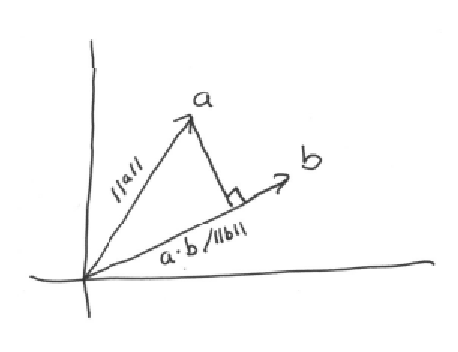
\includegraphics{projection.eps}

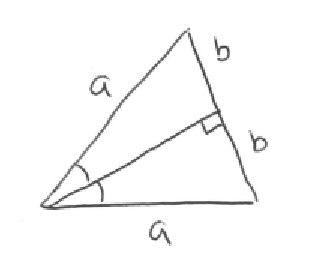
\includegraphics{isosoles_triangle.eps}

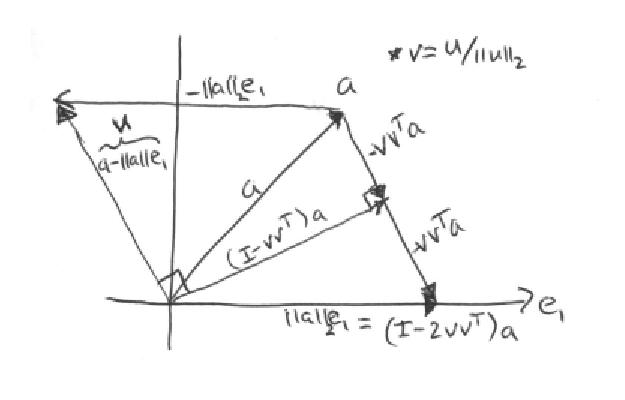
\includegraphics{householder.eps}


\section{Singular Value Decomposition}

The SVD is extremely stable and is in some sense the ultimate safe thing to do, if it is done right anyway.  We do not often do it as it is expensive (read slow) to calculate.  The danger in QR is in error buildup in solving, $R$, by back substitution.  It would be much nicer to have a diagonal matrix so errors couldn't buildup.  The SVD always exists and is a non-unique (i.e. there are many different SVD's for the same matrix) decomposition that is given by
\begin{eqnarray}
A &=& U\Sigma V^T
\end{eqnarray}
where $U$ and $V$ are unitary (generalization of orthogonal to complex numbers) matrices, and $\Sigma$ is  a diagonal matrix with the main diagonal ordered so $\sigma_1\geq\sigma_2\geq\cdots\geq\sigma_n\geq 0$.  Thus $\Sigma$ is not only diagonal, it is positive semidefinite (there could be zeros on the diagonal) and ordered.  We can even calculate individual singular values (the $\sigma_i$).  Some popular uses are
\begin{enumerate}
\item $\|A\|_2=\sigma_1$
\item $\|A^{-1}\|_2=\sigma_n^{-1}$
\item $cond(A)=\frac{\sigma_1}{\sigma_n}$
\item $\|A\|_{Frobenius}^2=\sum_{i=1}^n\sigma_i^2$
\item $A^{-1} = V\Sigma^{-1}U^T$, note $\Sigma^{-1}$ is easy to calculate because it is diagonal.
\end{enumerate} 
The fundamental theorem of Calculus tells us that an integral of a 
function can be expressed in terms of the anti-derivative of the 
function.  Unfortuneately, not all functions have anti-derivatives 
that are expressable in known functions.  One of the most famous is 
the Gaussian probability distribution, which is given by
\beqn
e^{-\left(\frac{x-\mu}{\sigma}\right)^{2}}.
\eeqn
The anti-derivative of this important and frequently occuring function 
is unknown.  How do we handle it?  That is the subject of this chapter.

\section{Riemann}
We recall from Calculus that the integral is defined as
\beqn
\int_{a}^{b}{f(x)dx} = 
\lim_{n\rightarrow\infty}\sum_{j=1}^{n}f(p_{j})(x_{j}-x_{j-1}).
\eeqn
Now assume that all $n$ of the $x_{j}$ are evenly spaced on $[a,b]$.  We 
can then write
\beqn
h & = & \frac{b-a}{n} \\
  & = & x_{j}-x_{j-1}.
\eeqn
We can use this to get an expression for the Riemann Sum
\beqn
\int_{a}^{b}{f(x)dx}
 & = & 
\lim_{n\rightarrow\infty}\sum_{j=1}^{n}f(p_{j})(x_{j}-x_{j-1}) \\
 & = & 
\lim_{n\rightarrow\infty}\sum_{j=1}^{n}f(p_{j})h \\
 & = & 
\lim_{n\rightarrow\infty}h\sum_{j=1}^{n}f(p_{j}).
\eeqn
To evaluate the integral numerically we are not able to take the 
limit, so we get
\beqn
\int_{a}^{b}{f(x)dx} 
 & \approx & 
h\sum_{j=1}^{n}f(p_{j}).
\eeqn
The exact size of $n$ for the approximation to be good is a key aspect 
of numerical integration.  Note also that I have not specified what 
$p_{j}$ is, as this form allows you to do a left, right, mid-point, 
maximum, or minimum.  The basic idea here is that we are approximating 
the function by a constant on the interval.

\setlength{\lll}{\textwidth}
\addtolength{\lll}{-2\fboxsep}
\addtolength{\lll}{-2\fboxrule}
\noindent
\fbox{%
\begin{minipage}{\lll}

\beqn
\int_{a}^{b}{f(x)dx} 
 & \approx & 
h\sum_{j=1}^{n}f(p_{j}).
\eeqn

\end{minipage}}

\chapter{Differentiation}

Numerical differentiation seems obvious.  In most introductions to calculus, the derivative is introduced as the limit of a series of secant lines.  Probably the most basic method of numerically taking the derivative is based off this formula.  It turns out that while it seems obvious, numerical derivatives are more difficult as we will see.

\section{Derivative Approximation}
Let's start at the basics, the two point method of obtaining the derivative is based off taking the derivative of the two point interpolation polynomial.
\beqn
f(x) & \approx &
   \frac{x_{1}-x}{h}f(x_{0})+\frac{x-x_{0}}{h}f(x_{1}) \\
f'(x) & \approx &
   \frac{-1}{h}f(x_{0})+\frac{1}{h}f(x_{1}) \\
 & = &
   \frac{f(x+h)-f(x)}{h}.
\eeqn
This is only exact when we take the limit as $h$ approaches zero.  We can see how the basic errors are dealt with by expanding the Taylor sequence.
\beqn
f(x+h)=f(x)+hf'(x)+\frac{h^{2}}{2}f''(c)
\eeqn
Using the Taylor series in the formula we obtain that the error in the
formula is
\beqn
E & = & f'(x)-\frac{f(x+h)-f(x)}{h} \\
& = & f'(x)-\frac{f(x)+hf'(x)+\frac{h^{2}}{2}f''(c)-f(x)}{h} \\
& = & f'(x)-\frac{hf'(x)+\frac{h^{2}}{2}f''(c)}{h} \\
& = & f'(x)-f'(x)+\frac{h}{2}f''(c) \\
& = & \frac{h}{2}f''(c).
\eeqn
Two other types of error occur.  First, there is subtractive difference errors.  We note that since $f(x)\approx f(x+h)$, when we
subtract them we will lose precision.  Second, there is error propagation.  Consider the fact that nothing we do in the real world is ever exact, so we actually measure and calculate a nearby solution:
\beqn
f(x) & = & \tilde{f}(x)+\epsilon_{1} \\
f(x+h) & = & \tilde{f}(x+h)+\epsilon_{2}.
\eeqn
Substituting this into our formula we find
\beqn
f'(x) & \approx &
   \frac{f(x+h)-f(x)}{h} \\
 & = &
   \frac{\tilde{f}(x+h)+\epsilon_{2}-\tilde{f}(x)+\epsilon_{1}}{h} \\
 & = &
   \frac{\tilde{f}(x+h)-\tilde{f}(x)}{h}+\frac{\epsilon_{2}-\epsilon_{1}}{h}.
\eeqn
The resulting error is
\beqn
E & = & f'(x)-\frac{f(x+h)-\epsilon_{2}-f(x)+\epsilon_{1}}{h} \\
& = & f'(x)-\frac{f(x)+hf'(x)+\frac{h^{2}}{2}f''(c)-\epsilon_{2}-f(x)+\epsilon_{1}}{h} \\
& = & f'(x)-\frac{hf'(x)+\frac{h^{2}}{2}f''(c)-\epsilon_{2}+\epsilon_{1}}{h} \\
& = & f'(x)-f'(x)+\frac{h}{2}f''(c)+\frac{\epsilon_{1}-\epsilon_{2}}{h} \\
& = & \frac{h}{2}f''(c)+\frac{\epsilon}{h}.
\eeqn
As long as the last term is non-zero, which it will be in general, if $h$ gets to small them the propagation errors dominate, see Figure~\ref{f-derivative_error}.  This is the real problem.  We did not have this problem with numerical integration because we were multiplying by $h$ rather than dividing by it.  The problem is more pronounced with higher order derivatives where you will be dividing by powers of $h$.  This problem motivates the use of integral equations rather than differential ones.  Unfortunately many integral equations are very ill-conditioned.  Anyway, the key idea is that there is a competition between several error types.


\begin{figure}
 \begin{center}
  \begin{lpic}{derivative_error(.5,.5)}
   \lbl[l]{2,75,90;Error}
   \lbl[b]{110,2,0;h}
  \end{lpic}
  \caption{Error in calculating the step size for different step sizes, $h$, for $f''(c)=2$ and $\epsilon=10^{-6}$.}\label{f-derivative_error}
 \end{center}
\end{figure}

\section{Tangent Line}

As of yet we have considered calculating the derivative from above.  Let us consider the derivative from below, and we will solve for it using the equation of a line and noting that the slope of the tangent line in the limit as $h=0$ is the derivative\footnote{We could have just used the same method we used in the last section, but what fun is that?}.
\beqn
y &=& mx+b \\
\eeqn
thus
\beqn
f(x) &=& mx+b \\
f(x-h) &=& m(x-h)+b.
\eeqn
Take the difference
\beqn
f(x)-f(x-h)
 &=& mx - m(x-h) \\
 &=& mh \\
m_{left} &=& \frac{f(x)-f(x-h)}{h}
\eeqn
This is the left approximation of the derivative and
\beqn
m_{right} &=& \frac{f(x+h)-f(x)}{h}
\eeqn
is the right approximation.  We get a better estimate by averaging them.
\beqn
m_{avg}
 &=&\frac{m_{left}+m_{right}}{2} \\
 &=&\frac{\frac{f(x)-f(x-h)}{h}+\frac{f(x+h)-f(x)}{h}}{2} \\
 &=&\frac{f(x)-f(x-h)+f(x+h)-f(x)}{2h} \\
 &=&\frac{f(x+h)-f(x-h)}{2h}
\eeqn
Interestingly the best thing we can do when we have three points is not to use the one we are trying to estimate the derivative of. The reason is, when we use the left approximation of the derivative, we are really estimating the derivative at $x-\frac{h}{2}$, and similarly for the right approximation.  By averaging we get an estimate of the derivative at $x$.

\section{Richardson Extrapolation}



\section{Higher Order Derivatives}

The second derivative is just the derivative of the first derivative.  Since the left and right approximations really give us the approximate derivative at $x\pm\frac{h}{2}$, we can use them, with their separation distance of $h$, to estimate the second derivative at $f(x)$.
\beqn
f''(x)
 &\approx& \frac{f'\left(x+\frac{h}{2}\right)-f'\left(x-\frac{h}{2}\right)}{h} \\
 &\approx& \frac{\frac{f(x+h)-f(x)}{h}-\frac{f(x)-f(x-h)}{h}}{h} \\
 &\approx& \frac{f(x+h)-2f(x)+f(x-h)}{h^2}
\eeqn
To solve for higher derivatives we will need more points: $f(x+2h)$, $f(x-2h)$, etc.  The further we go away the worse the approximation will be though, again showing that higher order derivatives become more inaccurate.

\subsection{Method of Undetermined Coefficients}

In addition to the point the derivative is to be evaluated at, we need one additional point per order of the derivative to be taken.  That is a first derivative takes 2 points, a second derivative takes 3 points, a third derivative takes 4, and so on.  Rather than memorize a bunch of formulas for higher powers, or even iterating the formula as above, we can use the method of undetermined coefficients, which can also be used for integration, interpolation, differential equations, etc.

Say we wanted to find the formula for the second derivative, which we know will require 3 points.
\begin{eqnarray*}
f''(x)=Af(x+h)+Bf(x)+Cf(x-h)
\end{eqnarray*}
We will use the Taylor Series to expand $f(x+h)$ and $f(x-h)$ around $x$.
\begin{eqnarray*}
f(x+h)=f(x)+hf'(x)+\frac{h^2}{2}f''(x)+hot \\
f(x-h)=f(x)-hf'(x)+\frac{h^2}{2}f''(x)+hot
\end{eqnarray*}
We now substitute this into the original expression.
\begin{eqnarray*}
f''(x)
&=&A\left(f(x)+hf'(x)+\frac{h^2}{2}f''(x)+hot\right)+Bf(x)+ \\
&&\qquad C\left(f(x)-hf'(x)+\frac{h^2}{2}f''(x)+hot\right) \\
&=& (A+B+C)f(x)+(A-C)hf'(x)+(A+C)\frac{h^2}{2}f''(x)+hot
\end{eqnarray*}
Equating like derivatives on the left and right we have

\begin{tabular}{ccc}
Derivative & Equation               & Implication \\\hline
$f(x)$     & $A+B+C=0$              & $B=-(A+C)$ \\
$f'(x)$    & $(A-C)h=0$             & $A=C$ \\
$f''(x)$   & $(A+C)\frac{h^2}{2}=1$ & $A=\frac{1}{h^2}$ \\
\end{tabular}

thus
\begin{eqnarray*}
f''(x)&=&\frac{1}{h^2}f(x+h)+\frac{-2}{h^2}f(x)+\frac{1}{h^2}f(x-h)\\
      &=&\frac{f(x+h)-2f(x)+f(x-h)}{h^2}.
\end{eqnarray*}
Note that we found the same formula a different way.

\chapter{Differential Equations}\label{c-DifEq}

Most practical problems will be described by a differential equation.
We will not in general know the form of the solution, but we usually
can find how they change with respect to each other.  From this basis
we would like to be able to find the actual solution.

\section{General Introduction}

Consider the general differential equation
\beq
\dot y(x)=f(x,y(x)). \label{DifEq-e1}
\eeq
Using basic calculus we see that the solution is given by
\beqn
y(x)=\int f(x,y(x))dx+c.
\eeqn
Often this is not very useful in solving equations however.  The way
to get practical solutions for this problem is covered in
differential equations, so I will just mention a few.

\subsection{Existence}
The problem~\ref{DifEq-e1} has a solution on an interval $x_{0}\leq x\leq
\min(b_{x},c)$ and $y_{0}\leq y\leq b_{y}$ if the function $f$ is continuous
on the interval for $c=\frac{\|y-y_{0}\|}{\max_{x,y}\left(\frac{\partial f(x,y)}
{\partial y}\right)}$.
\bfig
{\tt    \setlength{\unitlength}{0.92pt}
\begin{picture}(202,139)
\thinlines    \put(152,21){$c$}
              \put(155,104){\line(0,-1){73}}
              \put(40,31){\framebox(134,73){}}
              \put(40,31){\dashbox{5}(95,55){}}
              \put(135,85){\circle*{4}}
              \put(170,21){$b_x$}
              \put(28,101){$b_y$}
              \put(132,21){$x$}
              \put(33,82){$y$}
              \put(10,29){$y_0$}
              \put(38,12){$x_0$}
              \put(23,31){\vector(1,0){169}}
              \put(40,23){\vector(0,1){106}}
              \put(52,50){$f(x,y(x))$}
\end{picture}}
\efig{Existence requirements}{DifEq-f1}


\section{Euler's Method}

Euler was without a doubt one of the greatest mathematical minds to have ever lived.  He did work in almost every area you can imagine including numerical methods.  His method is simple and easy for people to use.  Unfortunately, as the old numerics folk theorem goes, ``that which is good for a person is bad for a computer and vise versa'' Euler's method is unstable numerically\footnote{The forward method actually, the backward method of Euler is stable though still far from a good method.}.  To introduce the method, say we knew a point, say $(x_0,y(x_0))$, we could denote our first point by the y-coordinate.
\beqn
y_{0} & = & y(x_0)
\eeqn
Now say we wanted to find the value of the function a short distance away, say at $x_0+h$.  It would be reasonable to do a first order taylor approximation.  Noting that $\dot y = f(x,y)$ allows us to write this in simple terms.
\beqn
y_{1} & = & y(x_{0}+h) \\
      & = & y_{0}+hf(x_{0},y_{0})
\eeqn
We could extend this process to find
\beqn
y_{n} & = & y(x_{0}+nh) \\
      & = & y_{n-1}+hf(x_{n-1},y_{n-1}) \\
      & = & y_{n-2}+hf(x_{n-2},y_{n-2})+hf(x_{n-2}+h,y_{n-2}+hf(x_{n-2},y_{n-2}))
\eeqn
Note that the third (last) term involves estimating based on an estimate.  It is here that the problem comes because the errors can build.  It is easier to show the problem by taking the \textit{Z}-Transform of the second line
\beqn
y_{n} & = & y_{n-1}+hf(x_{n-1},y_{n-1}) \\
Y & = & z^{-1}Y+hF(z^{-1}X,z^{-1}Y)
\eeqn
Assuming we are dealing with linear functions (a common assumption) we can pull the $z^{-1}$ out.
Error is given by
\beqn
Y(x)-y_{h}(x) & = & hD(x)+{\cal O}(h^{2}) \\
D'(x) & = & g(x)D(x)+\frac{1}{2}Y''(x), \qquad D(x_{o})=0 \\
g(x) & = & \left.\frac{\partial f(x,z)}{\partial z}\right|_{z=Y(x)}
\eeqn


\section{Runge-Kutta}

While Euler's method is nice and simple, it is far from the best.
Higher order Taylor methods can be derived but these require
evaluating multiple derivatives.  Even Richardson's extrapolation has
limits on its abilities.

Consider the Taylor series of $y$.
\beqn
y(x+h) & = & y(x)+hy'(x)+\frac{h^{2}}{2}y''(x)+\ldots \\
 & = & y(x)+hf(x,y)+\frac{h^{2}}{2}f'(x,y)+\ldots \\
 & = & y(x)+hf(x,y)+\frac{h^{2}}{2}\left(f_{x}(x,y)+f_{y}(x,y)f(x,y)\right)
        +\ldots \\
 & = & y(x)+hf(x,y)+\frac{h^{2}}{2}\left(f_{x}(x,y)+f_{y}(x,y)f(x,y)\right)
        +\ldots \\
 & = & y(x)+hf(x,y)+ah\left(\frac{h}{2a}f_{x}(x,y)+
           \frac{h}{2a}f(x,y)f_{y}(x,y)\right)
        +\ldots
\eeqn
Now we consider the Taylor series in two variables of $f(x,y)$.
\beqn
f(x+h,y+k) & = & \sum_{n=0}^{\infty}\frac{1}{n!}
 \left[h\frac{\partial}{\partial x}+k\frac{\partial}{\partial y}\right]^{n}f(x,y) \\
 & = & f(x,y)
 +\left[h\frac{\partial}{\partial x}+k\frac{\partial}{\partial y}\right]f(x,y)
 + \ldots \\
 & = & f(x,y)
 +hf_{x}(x,y)+kf_{y}(x,y)
 + \ldots
\eeqn
Rearranging we find
\beqn
f(x+h,y+k) -f(x,y)
  & = &
hf_{x}(x,y)+kf_{y}(x,y)
 + \ldots .
\eeqn
We use this in our Taylor series of $y$.
\beqn
y(x+h)
  & = & y(x)+hf(x,y)+ah\left(\frac{h}{2a}f_{x}(x,y)+\frac{h}{2a}f(x,y)f_{y}(x,y)\right)
        +\ldots \\
  & = & y(x)+hf(x,y)+h\left(af(x+\frac{h}{2a},y+\frac{h}{2a}f(x,y)) -af(x,y)\right)
        +\ldots \\
  & = & y(x)+h(1-a)f(x,y)+ahf(x+\frac{h}{2a},y+\frac{h}{2a}f(x,y))
        +\ldots \\
  & = & y(x)+h(1-a)f(x,y)+ahf(x+b,y+bf(x,y))
        +\ldots \\
& & \qquad b=\frac{h}{2a} \qquad 0\leq a \leq 1
\eeqn
We have defined this in order to take advantage of the many varieties
of second order R-K.  The most common are: Midpoint (a=1), Modified
Euler (a=1/2), and Heun's method (a=3/4).

You can also do R-K for higher orders.  The most common is fourth
order.  The algebra is tedious so I will just present the result.
\beqn
y(x+h) = y(x)+\frac{1}{6}\left(F_{1}+2F_{2}+2F_{3}+F_{4}\right)
\eeqn
with
\beqn
F_{1} & = & hf(x,y) \\
F_{2} & = & hf(x+\frac{h}{2},y+\frac{F_{1}}{2}) \\
F_{3} & = & hf(x+\frac{h}{2},y+\frac{F_{2}}{2}) \\
F_{4} & = & hf(x+h,y+F_{3})
\eeqn

\section{Fehlberg's Method}

We have seen that the local error (error in one step due mostly to
truncation) is one order of magnitude better than the global error,
in general.  Often we use Richardson's Error formula to find an
estimate of the local error ($T_{n}$) so we can adjust the step size
to keep things nice.  For instance Richardson's Error for Euler's
method gives us
\beqn
Y(x)-y_{h}(x) & \approx & hD(x) \\
Y(x)-y_{2h}(x) & \approx & 2hD(x) \\
Y(x)-y_{2h}(x) & \approx & 2(Y(x)-y_{h}(x)) \\
Y(x) & \approx & 2y_{h}(x)-y_{2h}(x) \\
Y(x)-y_{h}(x) & \approx & (2y_{h}(x)-y_{2h}(x))-y_{h}(x) \\
 & \approx & y_{h}(x)-y_{2h}(x).
\eeqn
This gives us a reasonable extrapolation formula, and estimate of the
error.  Another way to estimate the error would be to look at two
estimates from different order methods.  For instance you could do a
fourth and a fifth order R-K estimate at each step and use the
difference to bound the error.  If the error at any step became to
large then you would decrease the step size and try again.  This idea
is Fehlberg's method, and it is the basis of most modern ode solvers.
This is why Matlab has ode23 and ode45.

\section{Adams-Bashforth}

Up till now we have been looking at solving the differential equation
directly.  We could however just integrate both sides.
\beqn
y' & = & f(x,y) \\
\int_{x_{n}}^{x_{n+1}}y'dx & = & \int_{x_{n}}^{x_{n+1}}f(x,y)dx \\
y(x_{n+1})-y(x_{n}) & = & \int_{x_{n}}^{x_{n+1}}f(x,y)dx \\
y(x_{n+1}) & = & y(x_{n}) + \int_{x_{n}}^{x_{n+1}}f(x,y)dx
\eeqn
Our task is now reduced to trying to find the remaining integral,
which we can use the ideas we had from last chapter.  Adams-Bashforth
of order $m$ uses a polynomial approximation to $f(x,y)$ at the points
$x_{n}$, $x_{n-1}$, \ldots, $x_{n-m+1}$.  Consider the second order
Adams-Bashforth method.
\beqn
f(x,y(x)) & \approx &
  \frac{x_{n}-x}{h}f(x_{n-1})+\frac{x-x_{n-1}}{h}f(x_{n}) \\
\int_{x_{n}}^{x_{n+1}}f(x,y)dx & \approx &
  \int_{x_{n}}^{x_{n+1}}\left(
  \frac{x_{n}-x}{h}f(x_{n-1})+\frac{x-x_{n-1}}{h}f(x_{n})
  \right)dx \\
  & \approx &
  \left.
  \frac{x_{n}x-\frac{1}{2}x^{2}}{h}f(x_{n-1})+
  \frac{\frac{1}{2}x^{2}-x_{n-1}x}{h}f(x_{n})
  \right|_{x_{n}}^{x_{n+1}} \\
  & \approx &
  \frac{x_{n}h-\frac{x_{n+1}^{2}-x_{n}^{2}}{2}}{h}f(x_{n-1})+
  \frac{\frac{x_{n+1}^{2}-x_{n}^{2}}{2}-x_{n-1}h}{h}f(x_{n}) \\
  & \approx &
  \frac{x_{n}h-\frac{x_{n+1}^{2}-x_{n+1}x_{n}+x_{n+1}x_{n}-x_{n}^{2}}{2}}{h}f(x_{n-1}) \\
  & & \qquad +
  \frac{\frac{x_{n+1}^{2}-x_{n+1}x_{n}+x_{n+1}x_{n}-x_{n}^{2}}{2}-x_{n-1}h}{h}f(x_{n}) \\
  & \approx &
  \frac{x_{n}h-\frac{x_{n+1}h+x_{n}h}{2}}{h}f(x_{n-1})+
  \frac{\frac{x_{n+1}h+x_{n}h}{2}-x_{n-1}h}{h}f(x_{n}) \\
  & \approx &
  \frac{2x_{n}-(x_{n+1}+x_{n})}{2}f(x_{n-1})+
  \frac{x_{n+1}+x_{n}-2x_{n-1}}{2}f(x_{n}) \\
  & \approx &
  \frac{x_{n}-x_{n+1}}{2}f(x_{n-1})+
  \frac{x_{n+1}-x_{n-1}+x_{n}-x_{n-1}}{2}f(x_{n}) \\
  & \approx &
  \frac{-h}{2}f(x_{n-1})+\frac{2h+h}{2}f(x_{n}) \\
  & \approx &
  \frac{h}{2}(3f(x_{n})-f(x_{n-1}))
\eeqn
This is kind of ugly, so it would be nice to have a faster way of
handling things, especially as the dimensions increase.  Luckily there
is just such a technique.  The method of undetermined coefficients.  We start by assuming the general form we want, in this case,
\beqn
\int_{x_{n}}^{x_{n+1}}f(x,y)dx & \approx & af(x_n)+bf(x_{n-1}
\eeqn

We would like the approximation to work perfectly for constant and linear terms so:

Constant term, $f(x,y)=1$
\beqn
\int_{x_{n}}^{x_{n+1}}1dx & = & a\cdot 1+b\cdot 1 \\
h &=& a+b.
\eeqn

Linear term, $f(x,y)=x$
\beqn
\int_{x_{n}}^{x_{n+1}}xdx & = & a\cdot x_n+b\cdot x_{n-1} \\
\frac{x_{n+1}^2-x_n^2}{2} &=& a\cdot x_n-a\cdot x_{n-1}+a\cdot x_{n-1}+b\cdot x_{n-1} \\
\frac{x_{n+1}^2-x_nx_{n+1}+x_nx_{n+1}-x_n^2}{2} &=& a\cdot(x_n-x_{n-1})+(a+b)\cdot x_{n-1}.
\eeqn
Now noting that $a+b=h$
\beqn
\frac{x_{n+1}(x_{n+1}-x_n)+x_n(x_{n+1}-x_n)}{2} &=& a\cdot(h)+(h)\cdot x_{n-1} \\
\frac{x_{n+1}h+x_nh}{2} &=& a\cdot h+h\cdot x_{n-1} \\
\frac{x_{n+1}+x_n-2x_{n-1}}{2} &=& a \\
\frac{x_{n+1}-x_{n-1}+x_n-x_{n-1}}{2} &=& a \\
\frac{2h+h}{2} &=& a \\
\frac{3h}{2} &=& a.
\eeqn

Thus since $a+b=h$,
\beqn
b=\frac{-h}{2}
\eeqn
which is what we found before.

\section{Adams-Moulton}

Adams-Bashforth considered that we knew only up to $f(x,y)$ only at points up to $x_n$.  What if we assume we can use $x_n$ or a near approximation?  Let us again consider just the simple case of linear approximations to function, though we could use any order of polynomial we liked (if we want to do the work).
\beqn
f(x,y(x)) & \approx &
  \frac{x-x_{n}}{h}f(x_{n+1})+\frac{x_{n+1}-x}{h}f(x_{n})
\eeqn
Using this we can solve the integral.
\beqn
\int_{x_{n}}^{x_{n+1}}f(x,y)dx & \approx &
  \int_{x_{n}}^{x_{n+1}}\left(
  \frac{x-x_{n}}{h}f(x_{n+1})+\frac{x_{n+1}-x}{h}f(x_{n})
  \right)dx \\
  & \approx &
  \left.
  \frac{\frac{1}{2}x^{2}}{h}f(x_{n+1}-x_{n}x)+
  \frac{x_{n+1}x-\frac{1}{2}x^{2}}{h}f(x_{n})
  \right|_{x_{n}}^{x_{n+1}} \\
  & \approx &
  \frac{\frac{x_{n+1}^{2}-x_n^{2}}{2}-x_nx_{n+1}+x_n^2}{h}f(x_{n+1})+
  \frac{x_{n+1}^2-x_{n+1}x_n-\frac{x_{n+1}^{2}-x_n^{2}}{2}}{h}f(x_{n}) \\
  & \approx &
  \frac{x_{n+1}^{2}-x_n^{2}-2x_nx_{n+1}+2x_n^2}{2h}f(x_{n+1})+
  \frac{2x_{n+1}^2-2x_{n+1}x_n-x_{n+1}^{2}+x_n^{2}}{2h}f(x_{n}) \\
  & \approx &
  \frac{x_{n+1}^{2}-2x_nx_{n+1}+x_n^2}{2h}f(x_{n+1})+
  \frac{x_{n+1}^2-2x_{n+1}x_n-+x_n^{2}}{2h}f(x_{n}) \\
  & \approx &
  \frac{(x_{n+1}-x_n)^2}{2h}f(x_{n+1})+
  \frac{(x_{n+1}-x_n)^2}{2h}f(x_{n}) \\
  & \approx &
  \frac{h^2}{2h}f(x_{n+1})+\frac{h^2}{2h}f(x_{n}) \\
  & \approx &
  \frac{h}{2}(f(x_{n+1})+f(x_{n}))
\eeqn


\section{Stability \& Stiff Equations}
A good start for looking at stiff equations is to examine the
stability of our methods.  Consider Forward Euler for
\beqn
y'=-200y, \qquad y(1)=e^{-200}.
\eeqn
The solution can easily be seen to be $e^{-200x}$.  Forward Euler
gives us
\beqn
y_{i+1} & = & y_{i}-200*h*y_{i} \\
 & = & y_{i}(1-200*h).
\eeqn
We note that this is stable if $\| 1-200*h \|<1$.  Since $h>0$ we
must have $h<0.01$.  This is a smooth, monotonically decreasing
function that is less than $2\time10^{-87}$ and greater than zero.
Despite the smoothness and flatness, we have to take very small
steps.  To see this look at Figure~\ref{stabfig}.
\begin{figure}[h]
\begin{center}
\leavevmode
\hbox{
\epsfxsize=4in
\epsffile{stab.eps}}
\end{center}
\caption{Instability in Euler's Method}
\label{stabfig}
\end{figure}
Note that Backward Euler does not have the same problem.  It is
defined by
\beqn
y_{i+1} & = & y_{i}-200*h*y_{i+1} \\
 & = & y_{i}\frac{1}{1+200*h},
\eeqn
which is stable for all $h>0$. Stability is not the same thing as
stiffness, but they are related.  Stiffness is due to multiple scales
of the terms, for instance $e^{-x}$, $e^{-200x}$.  Consider the
following equation
\beqn
0=\ddot{y}+1001\dot{y}+1000y, \qquad y(0)=1, \qquad \dot{y}(0)=-1.
\eeqn
The solution can easily be seen to be $e^{-t}$, which is nice in any
definition.  We solve the equation using a 4th order R-K method.  The
results are in Figure~\ref{stifffig}.
\begin{figure}[h]
\begin{center}
\leavevmode
\hbox{
\epsfxsize=6in
\epsffile{stiff.eps}}
\end{center}
\caption{Stiff Equation}
\label{stifffig}
\end{figure}

What is going on?  We need to look at the eigenvalues.

Define the intermediate variable $z=\dot y$, and the equation becomes
\beqn
0&=&\dot z +1001z+1000y \\
\dot z&=&-1001z-1000y.
\eeqn
Putting this in matrix form
\beqn
\dot{\bmat y\\z \emat} &=&\bmat 0 & 1 \\ -1000 & -1001 \emat \bmat y\\z\emat
\eeqn
The eigenvalues are (-1,-1000).  Since the eigenvalues differ by three orders of magnitude we can expect stiffness, which is what Figure~\ref{stifffig} shows.


\input{KONA-ModSim.tex}
\input{KONA-PDE.tex}


\part{Numerical Linear Algebra}

\input{KONA-Spaces.tex}
\input{KONA-Matrix.tex}
\chapter{Four Fundamental Spaces}

\section{Definition}
\subsection{Domain}
\subsection{Range}
\subsection{Right Nullspace}
\subsection{Left Nullspace}
\subsection{Putting Them Together}

\section{SVD - Singular Value Decomposition}


\section{Inverse}

\subsection{Pseudo Inverse}
left inverse

right inverse

Moore-Penrose conditions

\subsection{Inverse}
A true inverse only exists when the matrix is square and full rank, in which case the matrix is said to be invertible.

\section{Projections}
\subsection{Properties}
Let $P_a$ be a projection onto the range of $a$.  If this is the case then projecting $a$ onto itself should not change anything.  Thus if I take any vector and project it onto the range of $a$ then project it onto the range of $a$ again, it should be the same as projecting onto the range of $a$ once.  Putting this formally,
\begin{eqnarray}
P_a(P_a x) & = & P_a x, \qquad\forall x\\
P_a^2 x & = & P_a x, \qquad\forall x\\
P_a^2 & = & P_a
\end{eqnarray}
When $P^2=P$, we say the matrix $P$ is idempotent, thus all projectors are idempotent.

If a projector is to be orthogonal it also has to be symmetric, since orthogonal projectors should provide an orthogonal basis for the space they project onto.

\subsection{Using SVD}
Now that we feel comfortable with the SVD, let's use it to solve a practical problem.

\appendix
\input{KONA-SciLab.tex}

\bibliographystyle{plain}
\bibliography{keithdis,keithcomp}

\end{document}
